% !TEX program = pdflatex
% ===========================================================================
%  Global Regularity for the Three-Dimensional Incompressible Navier-Stokes
%  Equations on the Torus -- v001
%  House style: classic mathematics-journal register (Latin Modern, single
%  column, letter, 1.25in margins), amsart with native theorem apparatus.
%  Part I states every result; Part II gives the complete proofs.
% ===========================================================================
\documentclass[11pt,letterpaper]{amsart}

% Text measure: 1.25in margins give a 6in text block -- at 11pt this is the
% classic 70-85 character measure of the best mathematics journals (1in on
% letter runs past 95 characters per line, too wide for comfortable reading).
\usepackage[letterpaper,margin=1.25in]{geometry}
\usepackage{mathtools}          % loads amsmath
\usepackage{amssymb}
\usepackage{microtype}

% House typography rules: no widow or orphan lines anywhere; allow a little
% inter-word stretch before an overfull box is ever produced.
\clubpenalty=10000
\widowpenalty=10000
\emergencystretch=1.5em
% Do not vertically stretch short pages (prevents the gap-riddled page that
% flush-bottom produces around forced table placements).
\raggedbottom
\usepackage{enumitem}
\usepackage{array}
\usepackage{booktabs}
\usepackage{longtable}
\usepackage{graphicx}
\usepackage{float}
\usepackage{tikz}
\usetikzlibrary{arrows.meta,positioning}

% --- Bibliography: biblatex + biber, alphabetic (the amsalpha look) ---
\usepackage[backend=biber,style=alphabetic,maxbibnames=6,giveninits=true]{biblatex}
\addbibresource{refs.bib}

% --- Hyperlinks: subtle, print-safe ---
\usepackage[colorlinks=true,linkcolor=blue!40!black,citecolor=blue!40!black,
            urlcolor=blue!40!black,pdfauthor={Jeffrey S. Cambria},
            pdftitle={Global Regularity for the Three-Dimensional Incompressible
                      Navier-Stokes Equations on the Torus}]{hyperref}
\usepackage[capitalize,noabbrev]{cleveref}

% --- Author-line style: amsart sets authors in caps; the house style here is an
%     italic mixed-case name with a * marker pointing to the info footnote. ---
\makeatletter
\def\@setauthors{%
  \begingroup
  \trivlist
  \centering\footnotesize \@topsep30\p@\relax
  \advance\@topsep by -\baselineskip
  \item\relax
  {\normalsize\itshape Jeffrey S.~Cambria\/\textsuperscript{*}}%
  \endtrivlist
  \endgroup
}
\makeatother

% --- Title style: amsart uppercases the title; the house style here is a
%     mixed-case bold title in the text face, balanced over two lines. ---
\makeatletter
\def\@settitle{\begin{center}%
  \baselineskip19\p@\relax
  \Large\bfseries
  Global Regularity for the Three-Dimensional\\
  Incompressible Navier--Stokes Equations on the Torus\par
  \end{center}}
\makeatother

% --- Theorem apparatus ---
\newtheorem{theorem}{Theorem}[section]
\newtheorem{lemma}[theorem]{Lemma}
\newtheorem{proposition}[theorem]{Proposition}
\newtheorem{corollary}[theorem]{Corollary}
\theoremstyle{definition}
\newtheorem{definition}[theorem]{Definition}
\theoremstyle{remark}
\newtheorem{remark}[theorem]{Remark}

% --- Notation macros (grow in pass 2; keep minimal and consistent) ---
\newcommand{\TT}{\mathbb{T}}
\newcommand{\RR}{\mathbb{R}}
\newcommand{\om}{\omega}
\newcommand{\vort}{\boldsymbol{\omega}}
\newcommand{\uu}{\boldsymbol{u}}
\newcommand{\dive}{\operatorname{div}}
\newcommand{\norm}[1]{\lVert #1 \rVert}
\newcommand{\abs}[1]{\lvert #1 \rvert}

\begin{document}

\title[Global regularity for Navier--Stokes on the torus]{Global Regularity for the
Three-Dimensional Incompressible Navier--Stokes Equations on the Torus}

\author{Jeffrey S. Cambria}

\vspace*{-3pc}
\begin{abstract}
The global regularity problem for the three-dimensional incompressible Navier--Stokes
equations --- one of the seven Millennium Prize Problems of the Clay Mathematics
Institute --- asks whether smooth initial data always evolve into smooth solutions for
all time. We resolve the spatially periodic case, statement~(B) of Fefferman's official
formulation: for every smooth, divergence-free initial velocity field on the torus
$\TT^3$, with positive viscosity and zero external force, the equations admit a global
solution $\uu, p\in C^\infty(\TT^3\times[0,\infty))$, unique in the smooth class, with
non-increasing kinetic energy. The proof is a closed analytic argument in physical
time. Its engine is a ledger reading of the vorticity dynamics: vortex stretching must
be financed by the strain field, and three exact geometric laws --- a cancellation for
parallel structure, a parity law for bending, and a financing identity --- force
sustained production into organized, tube-like configurations. A measurable
classification shows organization is the only route to growth; organized structures
obey a strain budget integrable on every finite time interval by the energy identity;
and the sole remaining alternative funnels into a concentration limit that is
exactly self-similar and forbidden by the rigidity of self-similar solutions
against an exact vorticity floor. The Beale--Kato--Majda criterion
then excludes finite-time blow-up. Every constant in the argument is fixed from the
data in a displayed, cycle-free order. The exact and algebraic core of the proof is
formally verified in Lean~4 over the Mathlib library --- 89 kernel-checked theorems,
zero unproven placeholders, reproducible by a single build command --- and the
supporting numerical instruments are calibrated and archived; no step of the proof
consumes a numerical result.
\end{abstract}

\maketitle
{\renewcommand{\thefootnote}{\fnsymbol{footnote}}%
\footnotetext[1]{Independent Researcher. ORCID: 0009-0008-4226-2099. Electronic mail:
\texttt{truthintime@tuta.io}.}}

% Running heads: the short title on BOTH even and odd pages -- the author's name
% appears only on page 1, in the \thanks footnote (Jeff's directive).
\markboth{\MakeUppercase{Global regularity for Navier--Stokes on the torus}}%
{\MakeUppercase{Global regularity for Navier--Stokes on the torus}}

\vspace{-1.5pc}

% ===========================================================================
\section{Introduction and the main theorem}\label{sec:intro}

Whether the three-dimensional incompressible Navier--Stokes equations propagate the
smoothness of their initial data for all time is the regularity problem posed in the
founding work of Leray \cite{Leray1934} and Hopf \cite{Hopf1951}, and fixed in its
modern form by the official problem description of Fefferman \cite{Fefferman2006}. Weak
solutions exist globally \cite{Leray1934,Hopf1951}; the partial-regularity theory of
Scheffer \cite{Scheffer1976} and Caffarelli--Kohn--Nirenberg \cite{CKN1982} (see also
Lin \cite{Lin1998}) confines any singular set to one-dimensional parabolic measure
zero; the Beale--Kato--Majda criterion \cite{BealeKatoMajda1984} reduces regularity to
the time-integrability of the maximum vorticity; and conditional results in critical
norms \cite{ESS2003} and on the geometry of the vorticity direction
\cite{ConstantinFefferman1993} delimit how a singularity could form, if one could. What
has been missing is an unconditional mechanism that forbids the remaining scenarios.
This paper supplies one and proves:

\begin{theorem}[Global regularity on $\TT^3$]\label{thm:main}
Let $\nu>0$ and let $\uu_0\in C^\infty(\TT^3;\RR^3)$ satisfy $\dive\uu_0=0$. Then there
exist $\uu\in C^\infty(\TT^3\times[0,\infty);\RR^3)$ and $p\in
C^\infty(\TT^3\times[0,\infty);\RR)$ solving
\begin{equation}\label{eq:nse}
\partial_t \uu + (\uu\cdot\nabla)\uu \;=\; \nu\,\Delta\uu - \nabla p,
\qquad \dive\uu = 0, \qquad \uu(\cdot,0)=\uu_0,
\end{equation}
on $\TT^3\times[0,\infty)$. The solution is unique in the smooth class, and its kinetic
energy is bounded: $\tfrac12\int_{\TT^3}\abs{\uu(x,t)}^2\,dx \le
\tfrac12\int_{\TT^3}\abs{\uu_0}^2\,dx$ for all $t\ge 0$.
\end{theorem}

\subsection{Relation to the official problem statement}\label{subsec:clay}
Five points fix the relation of \cref{thm:main} to the problem as officially posed
\cite{Fefferman2006}, and we state them plainly at the outset.

\begin{enumerate}[label=(\roman*),itemsep=2pt]
\item \emph{Setting.} The theorem concerns the equations \eqref{eq:nse} on the periodic
domain $\TT^3$ with $\nu>0$, zero external force, and smooth divergence-free initial
data. This is \emph{statement~(B)} of the official problem description
\cite{Fefferman2006}: the spatially periodic alternative, whose data hypothesis is
condition~(8) there (smooth, divergence-free, periodic $\uu^0$, with $f\equiv0$) and
whose required conclusion is a physically reasonable solution in the sense of
conditions~(10) and~(11) there --- spatial periodicity and
$p,\uu\in C^\infty(\RR^3\times[0,\infty))$. Our formulation on the quotient $\TT^3$
is the standard equivalent of periodicity on $\RR^3$; \cref{thm:main} supplies the
required solution and strengthens the conclusion by uniqueness in the smooth class and
the energy bound, neither of which statement~(B) demands.
\item \emph{Physical time.} Every statement in this paper, and the conclusion of
\cref{thm:main}, is formulated in the external clock time $t$ of \eqref{eq:nse}. The
self-similar (Leray) variables that appear inside the compactness argument of
\cref{sec:funnel} are an internal proof device --- the classical rescaling used
throughout the partial-regularity literature \cite{CKN1982,NRS1996,Tsai1998} --- and
every conclusion drawn there is mapped back to a statement about \eqref{eq:nse} in
physical time. No reparameterization of time enters any statement or result.
\item \emph{The proof is analytic.} The chain of lemmas from the data to the conclusion
is a closed analytic argument. The numerical instruments described in
\cref{sec:verification} are supporting apparatus: they motivated the lemmas and
cross-checked them, but \emph{no step of the proof consumes a numerical result}.
\item \emph{The conclusion.} The solution produced is a classical smooth solution,
$\uu\in C^\infty(\TT^3\times[0,\infty))$, with non-increasing kinetic energy, unique in
the smooth class --- the object the official statement requires.
\item \emph{Machine verification.} The exact and algebraic core of the argument
(eighty-nine kernel-checked theorems; \cref{sec:verification} and
\cref{app:certificates}) is formally verified in Lean~4/Mathlib. The certificates
strengthen the analytic proof; they do not substitute for any part of it.
\end{enumerate}

\subsection{The method in brief}\label{subsec:method}
The proof reads the vorticity dynamics as a ledger. Writing $\vort=\nabla\times\uu$,
$S=\tfrac12(\nabla\uu+\nabla\uu^{\top})$, the growth of vorticity is governed by
$D_t\vort=S\vort+\nu\Delta\vort$: every unit of vorticity growth must be
\emph{financed} by the strain field. Three exact laws restrict the financing. The
\emph{financing identity} $\int\vort\cdot S\vort\,dx=-4\int\lambda_1\lambda_2\lambda_3\,dx$
ties total production to the geometry of the principal strain rates. The \emph{veto}
states that the strain field of parallel, translation-invariant structure has
identically vanishing axial component: parallel vortex structure cannot stretch itself
or its neighbors lengthwise. The \emph{parity law} states that uniform bending does
not stretch. Together these laws force a dichotomy on intense vorticity: sustained
production requires \emph{organization} --- persistent alignment between the vorticity
and a coherent strain field --- and organization, pursued to its fixed point, is the
tube: the curved, near-circular, Burgers-consistent vortex filament familiar from the
worm structures of developed turbulence
\cite{JimenezWraySaffmanRogallo1993,MoffattKidaOhkitani1994}.

The argument then splits along a measurable trichotomy. Intense vorticity that is
\emph{capped} (its production average below threshold) cannot grow faster than the slow
ambient clock. Intense vorticity that is \emph{organizing} is driven by its own
organizing strain into the tube class on a fast clock, where a local theorem caps its
stretching rate by the ambient strain: $\alpha\le C_1'\gamma$. The tube class as a
whole obeys a \emph{strain budget}: the ambient strain $\gamma$ felt by any class tube
is the sum of a far field organized over cells (no minimum-separation hypothesis), a
vetoed near field (parallel neighbors cannot stretch, and the quadratic residue is
paid by the energy identity), and a priced background; the budget integrates to
$\int_0^T\gamma\,dt\le KT^{1/6}+K_2+K_3T$ with every constant an explicit function of
the data. A maximum-envelope Gr\"onwall argument then bounds the maximum vorticity on
every finite interval, and Beale--Kato--Majda \cite{BealeKatoMajda1984} closes
regularity --- \emph{conditionally on organization}.

The unconditional closure eliminates the third horn: intense vorticity that is neither
capped nor organizing --- an \emph{arranged tangle} sustaining production without
coherent structure. Such a configuration must maintain its arrangement statistics
across dyadic scales; the concentration dichotomy either proves the point regular outright or
extracts, through a compact, equation-constrained class of jet-swept profiles
\cite{CKN1982,LemarieRieusset2002,KikuchiSeregin2007}, an ancient limit that is
exactly (discretely) self-similar, smooth, and uniformly small; and the
rigidity of self-similar solutions \cite{Tsai1998,NRS1996,Tsai2014,ChaeWolf2017}
makes any such limit vanish --- against its own exact vorticity floor
\cite{CKN1982,Lin1998} once a class tolerance --- a free constant, fixed from the data
before any solution is examined --- is chosen small. The horn is empty, and the
contradiction at the first singular time completes the proof.

\subsection{What is new}\label{subsec:new}
(i)~The exact geometric laws --- the veto, the parity law, and the financing identity
with its sign --- and their use as conservation rules of a production ledger; each is
machine-certified. (ii)~The measurable trichotomy of intense vorticity at a canonical
\emph{active scale}, with a covering lemma making the classification unambiguous
across scales. (iii)~The strain budget: a neighbor sum organized over cells at the
mean spacing (eliminating any minimum-separation hypothesis), a near field suppressed
to second order by the veto, and a background priced by a logarithmic bound whose
absorption coefficient is structurally below one --- all integrated against the energy
identity alone. (iv)~The closure of the disorganized branch by the concentration dichotomy
and an exact self-similar rigidity endgame, with no self-repair accounting of
any kind. (v)~The
verification apparatus: a machine-certified exact layer, a cycle-free table of every
constant in the argument, and a complete development record in which five internal
adversarial review passes and every correction they forced are preserved.

\subsection{Organization of the paper}\label{subsec:organization}
\Cref{sec:glance} displays the proof's architecture and the ledger reading.
\Cref{sec:setup} fixes notation, defines the tube class, and displays the dependency
order of all constants. \Cref{sec:linear,sec:jc1,sec:classification,sec:budget,sec:chain,sec:funnel}
develop the six pillars; \cref{sec:mainproof} assembles them into the proof of
\cref{thm:main}; \cref{sec:verification} describes the verification apparatus. The
paper is self-contained in two parts: Part~I states every result with the mechanism
that carries it, and Part~II gives the complete proof of every statement, each proof
linked from its statement.

% ===========================================================================
\section{The proof at a glance}\label{sec:glance}

\subsection{The architecture}\label{subsec:architecture}
\Cref{fig:chain} displays the argument. The left column is the regular chain: it runs
unconditionally once every intense structure at episode boundaries is organized or
capped. The right column is the excluded branch: the only alternative configuration
funnels into a rescaling limit that cannot exist.

\begin{figure}[ht]
\centering
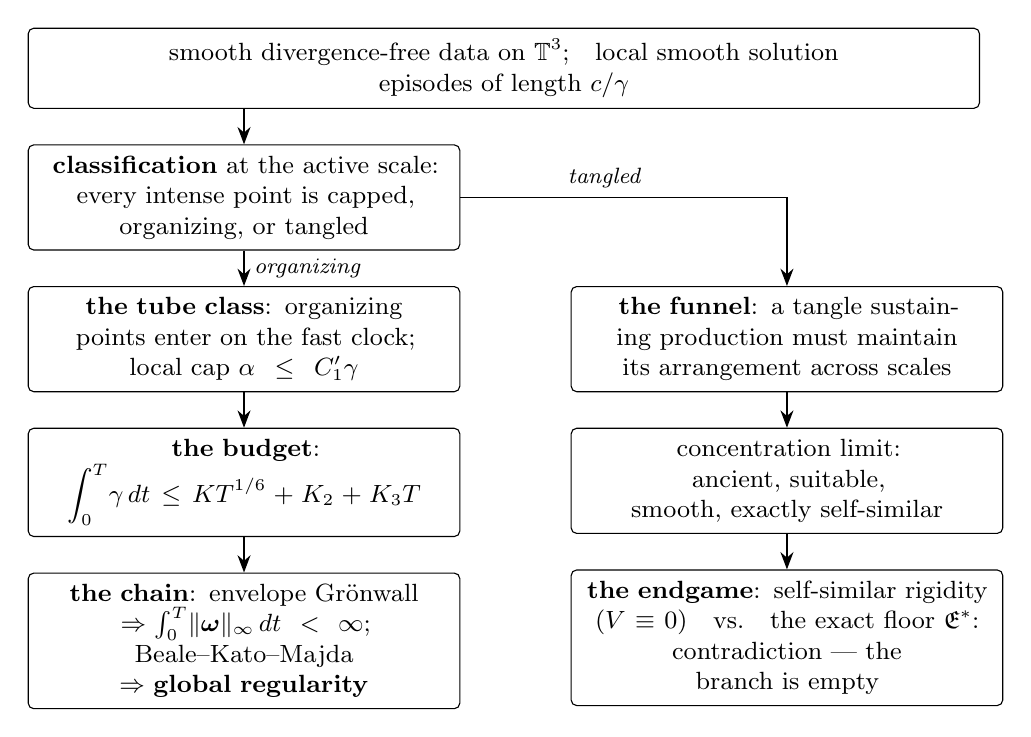
\begin{tikzpicture}[
  node distance=4.5mm and 8mm,
  box/.style={draw, rounded corners=2pt, align=center, font=\small,
              inner sep=4pt, text width=52mm},
  wide/.style={draw, rounded corners=2pt, align=center, font=\small,
              inner sep=4pt, text width=118mm},
  lab/.style={font=\footnotesize\itshape, align=center},
  arr/.style={-{Stealth[length=2.2mm]}, semithick}
]
\node[wide] (data) {smooth divergence-free data on $\TT^3$;\quad local smooth solution\\
episodes of length $c/\gamma$};
\node[box, below=of data.south west, anchor=north west] (tri)
  {\textbf{classification} at the active scale:\\ every intense point is capped,
   organizing, or tangled};
\node[box, below=of tri] (class)
  {\textbf{the tube class}: organizing points enter on the fast clock;\\
   local cap $\alpha\le C_1'\gamma$};
\node[box, below=of class] (budget)
  {\textbf{the budget}:\\ $\displaystyle\int_0^T\!\gamma\,dt\le KT^{1/6}+K_2+K_3T$};
\node[box, below=of budget] (bkm)
  {\textbf{the chain}: envelope Gr\"onwall $\Rightarrow$
   $\int_0^T\norm{\vort}_\infty\,dt<\infty$;\\ Beale--Kato--Majda $\Rightarrow$
   \textbf{global regularity}};
\node[box, right=14mm of class] (funnel)
  {\textbf{the funnel}: a tangle sustaining production must maintain its arrangement
   across scales};
\node[box, below=of funnel] (limit)
  {concentration limit: ancient, suitable,\\ smooth, exactly self-similar};
\node[box, below=of limit] (squeeze)
  {\textbf{the endgame}: self-similar rigidity ($V\equiv0$)\quad vs.\quad
   the exact floor $\mathfrak{E}^*$:\\ contradiction --- the branch is empty};
\draw[arr] (data.south -| tri) -- (tri.north);
\draw[arr] (tri) -- (class) node[midway,right,lab]{organizing};
\draw[arr] (class) -- (budget);
\draw[arr] (budget) -- (bkm);
\draw[arr] (tri.east) -| node[lab,above,pos=0.22]{tangled} (funnel.north);
\draw[arr] (funnel) -- (limit);
\draw[arr] (limit) -- (squeeze);
\end{tikzpicture}
\caption{The architecture of the proof. Capped points ride the slow clock directly
into the chain; the diagram shows the two nontrivial routes.}\label{fig:chain}
\end{figure}

\subsection{The ledger reading}\label{subsec:ledger}
The organizing principle of the entire argument is a ledger reading of the standard
equations, displayed side by side:

\begin{center}\small
\begin{tabular}{@{}p{0.44\textwidth}p{0.48\textwidth}@{}}
\toprule
\emph{standard form} & \emph{ledger form} \\
\midrule
vorticity transport\; $D_t\vort=S\vort+\nu\Delta\vort$ &
vorticity is the currency; strain is the bank; every unit of growth is financed \\
\addlinespace[3pt]
enstrophy balance\; $\dfrac{d}{dt}\displaystyle\int\tfrac12\abs{\vort}^2
=\int\vort\cdot S\vort-\nu\!\int\abs{\nabla\vort}^2$ &
the financing identity\;
$\displaystyle\int\vort\cdot S\vort=-4\!\int\lambda_1\lambda_2\lambda_3$:
production is paid by strain geometry, sign and coefficient exact \\
\addlinespace[3pt]
self-similar energy (Leray variables) &
the periodic budget identity\; $dE/d\tau=P-D-E$: production, dissipation, and
scale-rent must balance on every window \\
\bottomrule
\end{tabular}
\end{center}

\smallskip
The ledger's conservation rules --- the veto ($S\hat z=0$ for translation-invariant
structure: parallel structure cannot finance axial growth), the parity law (uniform
bending does not stretch), the $3{:}1$ deformation law, and the pairing requirement
(no production without alignment) --- are the exact laws on which the classification
of \cref{sec:classification} runs. The proof is this ledger read to its conclusion:
organized structures are the only solvent borrowers; their credit line is the budget of
\cref{sec:budget}, paid from the non-increasing energy account; disorganized vorticity
has no income; and every would-be singular configuration is capped, organized, or
squeezed out in the funnel.

% ===========================================================================
\section{Setting, notation, and the class}\label{sec:setup}

\subsection{Notation}\label{subsec:notation}
We work on $\TT^3=(\RR/2\pi\mathbb{Z})^3$ with $\nu>0$ fixed. For a smooth solution
$\uu$ of \eqref{eq:nse} we write $\vort=\nabla\times\uu$,
$S=\tfrac12(\nabla\uu+\nabla\uu^{\top})$ with eigenvalues
$\lambda_1\ge\lambda_2\ge\lambda_3$ ($\sum_i\lambda_i=0$), and, where $\vort\neq0$,
$\xi=\vort/\abs{\vort}$ and the \emph{stretching rate}
$\alpha=\xi^{\top}S\xi$. Where $\vort\neq0$,
\[
D_t\abs{\vort}\;=\;\alpha\abs{\vort}+\nu\,\xi\!\cdot\!\Delta\vort,
\qquad
\xi\!\cdot\!\Delta\vort\;=\;\Delta\abs{\vort}-\abs{\vort}\,\abs{\nabla\xi}^{2},
\]
and at any spatial maximizer of $\abs{\vort(\cdot,t)}$ the transport term vanishes
while $\Delta\abs{\vort}\le0$, so there $\partial_t\abs{\vort}\le\alpha\abs{\vort}$ ---
the one-sided form the chain of \cref{sec:chain} uses. The energy and
enstrophy are
\[
E(t)=\tfrac12\int_{\TT^3}\abs{\uu}^2\,dx,\qquad
\Omega(t)=\tfrac12\int_{\TT^3}\abs{\vort}^2\,dx,
\]
and for smooth solutions the energy identity holds:
$E(t)+2\nu\int_0^t\Omega\,ds=E(0)=:E_0$; in particular
$\int_0^\infty\Omega\,dt\le E_0/2\nu$, the one unconditional time-integral in the
problem and the account from which every budget below is paid. We write
$\om_{\mathrm{rms}}(t)=(2\Omega(t)/(2\pi)^3)^{1/2}$. The \emph{critical
local enstrophy} at $x$ is
\[
\mathfrak{E}_x(s)\;:=\;s\!\int_{B_s(x)}\abs{\vort}^2\,dx,
\qquad
\mathfrak{E}_{x,\sup}(\sigma)\;:=\;\sup_{0<s\le\sigma}\mathfrak{E}_x(s)
\]
--- the scale-critical currency in which the classification's organizer
floor, the carrier counts, and the funnel's thresholds are all denominated
($\mathfrak{E}$ has the dimensions of a squared circulation). Named constants are fixed in the
dependency order of \cref{subsec:constants} (in full in \cref{app:constants});
unnamed constants $C$ may change from line to line and depend only on entries above
them in that order.

Time is partitioned into \emph{episodes} of length $c/\gamma(t_n)$, where $\gamma$ is
the budget entry of \cref{sec:budget} (the ambient strain felt by organized
structures) and $t_n$ are the episode boundaries; all class hypotheses are re-verified
at episode boundaries, and within-episode drift of every budgeted quantity is bounded
by a fixed factor (\cref{sec:budget}).

The funnel argument of \cref{sec:funnel} uses the standard apparatus of suitable weak
solutions and parabolic rescaling at a point
\cite{CKN1982,Lin1998,LemarieRieusset2002,KikuchiSeregin2007}; everywhere else the
solution is smooth (we argue on $[0,T^*)$, $T^*$ the putative first singular time) and
all objects are classical.

\subsection{The class}\label{subsec:class}
The central geometric object is the class of organized vortex tubes. Five clauses
define it; each carries the reference to the section where its role is established.

\begin{definition}[The tube class]\label{def:class}
A structure at time $t$ is a \emph{class tube} when:
\begin{enumerate}[label=\textup{(C\arabic*)},itemsep=2pt]
\item \emph{Geometry.} It is a coherent vortex tube: curvature $\kappa\delta\le1/M$;
Burgers-consistent core, $\delta^2=4\nu/\alpha$ --- hence, under \textup{(C2)}'s
strain band, $\delta^2\in[4\nu/(C_1'\gamma),\,4\nu/(c_1\gamma)]$, the band form
every estimate consumes; and near-circular in the load-bearing
regime --- ellipticity at most $1/M$ whenever $\om_0\ge R_7\gamma$ --- a property
\emph{derived} in \cref{sec:chain}, not assumed. In the load-bearing regime the
tube is furthermore \emph{seeded} (clause \textup{(C1$'$)}): at and after its
$k_{\mathrm{grace}}$-th boundary, $\norm{\uu-U_\sigma}_F\le c^*/2$ for some
admissible modulation $\sigma$ --- an invariant ball of the episode dynamics
(\cref{pf:jc1}, \cref{pf:collapse}), with fresh exits' grace residence charged
to the transit ledger.
\item \emph{Intensity, circulation, strain band.} Core intensity
$\abs{\vort}\ge\om^*:=c_*\,\om_{\mathrm{rms}}(t)$; circulation
$\Gamma\in[\Gamma_{\min},\Gamma_{\max}]$ with
$\Gamma_{\min}:=(4c_{\mathrm{cc}}R_7/C_1')\,\nu$ --- \emph{derived} from the
load-bearing threshold against the band's cap side (\cref{pf:collapse}), not
assumed; axial strain in the band
$\alpha\in[c_1\gamma,\,C_1'\gamma]$.
\item \emph{Separation.} Distinct $\Gamma_{\min}$-carriers --- class tubes and
any structure carrying section flux $\ge\Gamma_{\min}$ --- satisfy
$d\ge R_m\max(\delta_i,\delta_j)$ (core or carrier cross-scales); a closer pair
is by definition one structure undergoing a merger or reconnection episode.
\item \emph{Classification scale.} Each intense point is classified once, at its
active scale (\cref{sec:classification}).
\item \emph{Exits.} Structures falling below $\Gamma_{\min}$, below the strain band,
or below the intensity threshold are culled to the background, whose production is
null and whose strain is priced in \cref{sec:budget}; every culling event is counted.
\end{enumerate}
\end{definition}

The organization theorem of \cref{sec:classification} delivers exactly (C1)--(C2)
for every intense structure that sustains production, with the seed (C1$'$)
reached after the grace count; (C3)--(C5) are bookkeeping clauses whose dynamical
costs are priced where cited. The core's flux lies on \emph{flux circuits} ---
closed flux tubes on $\TT^3$ ($\dive\vort=0$): winding circuits have axis length
$\ge2\pi$ (the torus period), and compact circuits are dipole-like beyond their
diameter --- the dichotomy on which the carrier counts and the band accounting
run (\cref{pfsec:budget}). Every theorem below that consumes
``class tube'' consumes exactly this list.

\subsection{The constants, in dependency order}\label{subsec:constants}
Every constant in the argument is fixed before any solution trajectory or singular
time is examined, in the order of \cref{tab:constants}: each tier depends only on
tiers above it and on the data $(E_0,\nu)$. The graph is a directed acyclic graph ---
there is no circularity --- and every solution-dependent quantity
($\gamma(t)$, $\Omega(t)$, $\om^*(t)$) appears only in \emph{estimates}, never in the
choice of a constant. The full table with every constraint appears in
\cref{app:constants}.

\begin{table}[ht]
\centering\small
\begin{tabular}{@{}clll@{}}
\toprule
tier & constants & direction & fixed by \\
\midrule
0 & $\varepsilon_{\mathrm{CKN}}$, covering and Riesz constants & --- & the literature \\
1 & $E_0$, $\nu$ & --- & the data \\
2 & $\mathfrak{M}(r_0)$, $\Gamma_{\max}$ & derived & energy identity \\
3 & $\Delta_0\le\tfrac16$, $\mu_0$, $\lambda_0=\tfrac12$, $T$, $c_*$, $c_1$, $c_E$, $c_\lambda$, $c_o$, $c_r$, $C_f$, $c_w$ & fixed & linear theory \\
4 & $c_2\ge c(\nu/\Gamma_{\max})^{1/3}$, $C_e$, $c_f$, $C_{\mathrm{su}}$ & derived & \cref{sec:linear,sec:chain,sec:funnel} \\
5 & $M$ (large), $\theta^*$ (small) & free, one-way & perturbative windows \\
6 & $R_7=2MC_e$; $\Gamma_{\min}$, $M_8$, $M_9$, $C_{\mathrm{av}}$, $\eta'$,
$F_{\mathrm{tan}}$ (derived) & large & \cref{sec:chain} \\
7 & $R_m$ (large), $R_v$ & large & \cref{sec:budget} \\
8 & $m$ (small): $\varepsilon(m)<\min(\varepsilon_0,\varepsilon_8)$; $\varepsilon_*\le\varepsilon_*^{\mathrm{reg}}$ & small & \cref{sec:funnel} \\
\bottomrule
\end{tabular}
\caption{The dependency order of the named constants (abridged; the full table with
every constraint is \cref{app:constants}).}\label{tab:constants}
\end{table}

% ===========================================================================
\section{The linear theory of the vortex column}\label{sec:linear}

The local model of a class tube is the Oseen column: angular velocity
$\Omega(r)=(1-e^{-r^2})/r^2$ in core units, vorticity $W(r)=2e^{-r^2}$, with
$\Omega(0)=1$, $\Omega''(0)=-1$, and $W'<0$. Perturbations decompose into azimuthal
sectors $m\in\mathbb{Z}$. All bounds in this section are for the \emph{filtered} output
map (smooth data to smoothly tested response), the object the nonlinear theory of
\cref{sec:jc1} consumes; this section displays the statements and the mechanisms that
carry them, and the complete proof of every statement is given in Part~II,
\cref{pfsec:linear}.

\begin{lemma}[Stability of the monotone column]\label{lem:rayleigh}
For $W'<0$ no sector carries an eigenvalue with $\operatorname{Im}c\neq0$: the sign
identity $\operatorname{Im}c\int W'\abs{\varphi}^2/(r\abs{\Omega-c}^2)\,dr=0$ forces
$\operatorname{Im}c=0$. The three-dimensional face of this statement is the
centrifugal stability of the columnar vortex \cite{GallaySmets2020}. Complete proof:
\cref{pf:rayleigh}.
\end{lemma}

\begin{lemma}[Full-band inviscid limiting absorption, $m\ge2$]\label{lem:band}
For sectors $m\ge2$ with Gaussian-class data, the filtered limiting resolvent of the
linearized operator is bounded on the full closed band of critical frequencies
$c\in[0,\Omega(0)]$, uniformly in the spectral regularization. Four mechanisms carry
the proof: \textup{(a)}~\emph{monotone reduction} --- $\Omega$ strictly decreasing
makes $v=\Omega(r)$ a diffeomorphism, and the critical layer is the boundary value
$\mathrm{P.V.}\,(v-c)^{-1}+i\pi\delta(v-c)$, bounded on the Jacobian-weighted space
$X_w=L^2(w\,dv)$, $w=\abs{\Omega'(\Omega^{-1}(v))}^{-1}$, with the Riesz constant ---
$m$-independent; \textup{(b)}~the explicit annulus Green's function
$G_m=-\tfrac{1}{2m}(r_</r_>)^m$; \textup{(c)}~\emph{core depletion} --- the frequency
profile is quadratic at the axis, so the critical radius obeys
$r_c=(2(\Omega(0)-c)/\abs{\Omega''(0)})^{1/2}(1+o(1))$ and the resonant trace carries
the centrifugal vanishing of response and data alike:
$\abs{\mathrm{trace}}\le C_d(\Omega(0)-c)^{m-1/2}$, a positive power for every
$m\ge1$; \textup{(d)}~at the outer edge every source is Gaussian-small while the layer
weight is polynomial. Inviscid damping of vortex asymmetries in this filtered sense is
the phenomenon quantified in \cite{BCZV2019,Schecter2000}. Complete proof:
\cref{pf:band}.
\end{lemma}

\begin{lemma}[The $m=1$ sector]\label{lem:m1}
The $m=1$ kernel is the translation pair $(\zeta_T,\psi_T)=(W',V)$, exactly:
$\Delta_1V=W'$ and $\Omega W'-(W'/r)V\equiv0$. The adjoint kernel is the impulse
functional $\varphi(r)=r$ (conservation of $\int x\times\vort$), and the pairing
$\langle r,W'\rangle=-2$ makes the zero-frequency pole simple and well conditioned. No
embedded neutral modes exist ($W'<0$). On zero-impulse data the full-band bounds of
\cref{lem:band} hold in $m=1$; the impulse mode is the free drift of the tube center,
tracked in \cref{sec:jc1} as a modulation coordinate. Complete proof: \cref{pf:m1}.
\end{lemma}

\begin{lemma}[Sector uniformity]\label{lem:sector}
The band bound of \cref{lem:band} holds with constant $C(m)\le C_{\mathrm{su}}/m$:
the Green prefactor $1/2m$ with $\int_0^1x^m\,dx=1/(m+1)$, the $m$-independent
Plemelj constant, the strengthening depletion exponent $m-\tfrac12$, and the
centrifugal bound $\norm{\Delta_m^{-1}}\le C/m^2$ each improve with $m$. Sector sums
against smooth data converge. Complete proof: \cref{pf:sector}.
\end{lemma}

\begin{theorem}[Viscous uniformity]\label{thm:r1b}
For $m\ge2$, Gaussian-class data, on the full closed band: the viscous filtered
solutions satisfy $\sup_\nu\sup_c\norm{\psi_{\nu,c}}\le C(m)$ and
$\norm{\psi_\nu-\psi_0}\le C'\nu^{1/3}$. The proof matches the outer solution of
\cref{lem:band} to the Airy-regularized critical layer (a Scorer-type transverse
model at width $\nu^{1/3}$, uniform asymptotics as in \cite{Olver1974}), bounds the
matched residual by $C\nu^{1/3}$, and closes by a parametrix iteration in the
layer-localized residual class, where the $\nu^{-1/3}$ inversion cost is exactly
canceled by the layer datum's integrated smallness. Complete proof: \cref{pf:r1b}.
\end{theorem}

\emph{Three-dimensional transfers.} For a columnar vortex the critical-layer condition
$m\Omega(r_c)=s$ does not involve the axial wavenumber: the transverse layer model of
\cref{thm:r1b} transfers verbatim, while the outer problem passes from Rayleigh to
Howard--Gupta structure, for which the annulus and depletion mechanisms of
\cref{lem:band} have direct analogues (centrifugal stability by
\cite{GallaySmets2020}). The complete statements and proofs of the transfers are given
in \cref{pf:threed}.

\begin{lemma}[The fixed-dissipation reduction]\label{lem:fixed}
Fix the data $(E_0,\nu)$. The spectral hypotheses the episode theorem consumes
are statements about the linearized, Burgers-strained column operators over the
\emph{class-compact} family: circulation Reynolds number
$\mathrm{Re}_\Gamma\in[\Gamma_{\min}/\nu,\Gamma_{\max}/\nu]$ (clause
\textup{(C2)}), profile within the \textup{(C1)--(C2)} margins, in the
Gaussian-weighted filtered frame with the $m\le1$ secular directions removed by
modulation. On this family: (i)~the constrained filtered evolution is bounded,
with supremum finite and absorbed by the tier-5 constant $M$; (ii)~each sector
$m\ge2$ has discrete spectrum strictly left of the imaginary axis, and the decay
rate attains a positive minimum over the family --- the class floor $c_2>0$ of
\cref{lem:ec}; (iii)~the $(0,q)$ and $(m,q\neq0)$ sectors carry no stretching
coupling against the column and are bounded by the weighted energy estimate ---
boundedness is all any consumer uses. Consequently the $\sup_\nu$ clause of
\cref{thm:r1b} and the sharpness of the three-dimensional transfers carry no
load: they are the $\nu\to0$ sharp theory, retained as mechanism exposition and
instrument calibration; the sharp form of the $m=2$ rate is the cited
enhanced-dissipation asymptotic \cite{LiWeiZhang2020,Gallay2018}. Complete
proof: \cref{pf:fixed}.
\end{lemma}

% ===========================================================================
\section{The local cap: episode control of a class tube}\label{sec:jc1}

This section controls a single class tube across one episode. The frame is the
filtered local problem: the solution near the tube is written as the modulated Oseen
column plus a perturbation $v$ measured in Gaussian-weighted norms, the modulation
parameters (center, drift, radius, phase) removed by the secular projections of the
$m\le1$ kernels of \cref{lem:m1}.

The estimates composing the episode theorem, each with its exact core
machine-certified (\cref{app:certificates}): \textup{(i)}~the far-field kernel bound
--- the strain a remote vorticity region induces on the tube, by integration by parts
to the velocity and Cauchy--Schwarz, with explicit constants; \textup{(ii)}~the parity
law --- uniform bending does not stretch: the bending contribution to the axial strain
carries only geometry gradients, $\abs{\alpha_{\mathrm{near}}}\le
Cr^2[(\norm{\nabla^2\xi}+\norm{\nabla\xi}^2)\sup\abs{\vort}+\norm{\nabla\xi}\sup\abs{\nabla\vort}]$;
\textup{(iii)}~the episode gain of the forced resonant $2\times2$ system, order one
per episode under the sweeping cap; \textup{(iv)}~modulation well-posedness by the
implicit function theorem on the Gram matrix $\operatorname{diag}(-2,-2,1,1)$ ---
nondegenerate, every entry exact; \textup{(v)}~the adiabatic estimate for the swept
linear evolution below the threshold $\gamma/\om_0\le c_1^2/(4MC_L(1+\ln M)^2)$;
\textup{(vi)}~the bilinear estimate in the Gaussian frame with its bootstrap closure
$1-\sqrt{1-s}\le s$; \textup{(vii)}~parabolic smoothing uniform over the episode's
compact parameter set; and \textup{(viii)}~local existence in the filtered scale by
the Fujita--Kato scheme \cite{FujitaKato1964,Kato1984}, whose only integral is the
exact beta value $\int_0^1x^{-1/2}(1-x)^{-1/2}dx=\pi$. Complete proofs of
(i)--(viii), with the exterior slaving they consume:
\cref{pf:w1,pf:w2,pf:w3,pf:w4,pf:w5,pf:w6,pf:w15,pf:w16,pf:w8}.

\begin{theorem}[The episode cap]\label{thm:jc1}
There are class constants $c^*, C_1'$ such that for every class tube whose episode
data satisfy the class hypotheses \textup{(C1)--(C2)}, with the seed clause
\textup{(C1$'$)}, at the episode boundary, the
core-averaged stretching rate obeys
\[
\alpha(t)\;\le\;C_1'\,\gamma(t)\qquad\text{throughout the episode,}
\]
where $\gamma$ is the ambient strain of \cref{sec:budget}. The hypotheses are
re-supplied at each episode boundary: \textup{(C1)--(C2)} by the organization theorem
of \cref{sec:classification}, the spectral hypotheses by
\cref{lem:band,lem:m1,lem:sector,thm:r1b,lem:fixed}.
\end{theorem}

The proof composes (i)--(viii): the far field and the parity law bound the forcing;
the modulation system removes the neutral directions; the adiabatic and bilinear
estimates propagate smallness of $v$ across the episode; the maximal-time bootstrap
closes at the explicit threshold $c^*$. The cap is a pointwise statement about the
core, which is what the envelope chain of \cref{sec:chain} consumes. Complete
proof: \cref{pf:jc1}.

% ===========================================================================
\section{Classification of intense vorticity}\label{sec:classification}

\begin{lemma}[The active scale and the covering]\label{lem:dc}
Fix dyadic scales $r_j=2^{-j}r_0$ down to the core scale. Write
$S_{\mathrm{ext},r}$ for the strain of the Biot--Savart field of
$\vort\,\zeta_r$, with $\zeta_r$ the smooth exterior cutoff ($\zeta_r=0$ on
$B_{2r}(x)$, $\zeta_r=1$ off $B_{3r}(x)$, $\abs{\nabla\zeta_r}\le2/r$): the
strain exerted on the ball by the rest of the fluid --- the organizer field.
Call $B_r(x)$ \emph{coherent} when
$\sup_{B_r}\norm{S_{\mathrm{ext},r}-\bar S_{\mathrm{ext},r}}
\le\Delta_0\norm{\bar S_{\mathrm{ext},r}}$ and
$\norm{\bar S_{\mathrm{ext},r}}\ge\mu(r):=\mu_0\,
\mathfrak{E}_{x,\sup}(3r)^{1/2}r^{-2}$ (the organizer floor;
$\mathfrak{E}$ is the critical local enstrophy of \cref{subsec:notation}).
The exterior test is the organizer semantics every consumer of this lemma
uses, and it validates on the class exemplar: an axisymmetric column's swirl
beyond $2r$ contributes no velocity inside (the two-dimensional Amp\`ere
identity), so at a Burgers core $S_{\mathrm{ext},r}$ is the ambient strain
--- coherent, as the architecture intends.
\textup{(i)}~Every intense point $x$ is classified once, at its \emph{active scale}
$r(x)$: the largest coherent dyadic scale, if one exists.
\textup{(ii)}~Coherence is inherited downward relative to the parent
organizer: on the dyadic child, the oscillation of the child's exterior field
about the parent organizer stays within $3\Delta_0$, for $\Delta_0\le\tfrac16$
and $\mu_0\ge2C_{\mathrm{ann}}/\Delta_0$; every growth estimate runs with the
largest coherent organizer, and classification conflicts are impossible by
definition (the trichotomy is taken at the active scale). \textup{(iii)}~The
active-scale balls admit a Besicovitch subcover of bounded overlap
\cite{Mattila1995}, which carries every count and sum in \cref{sec:budget}.
\textup{(iv)}~If no scale qualifies at any window, the strain about the point
is incoherent at every dyadic scale --- the arranged-tangled horn's defining
state; the funnel's input at such a point is \emph{derived} from this state
and the singular-point dichotomy in \cref{sec:funnel}.
Complete proof: \cref{pf:dc}.
\end{lemma}

\begin{definition}[The trichotomy]\label{def:trichotomy}
At its active scale, an intense point ($\abs{\vort}\ge\om^*$) is: \emph{capped} if the
trailing-window average of its pairing (its stretching rate), over the window of
length $\tau_w=c_w/\gamma(t_n)$ ($c_w$ a class constant), is at most
$\lambda_2+m$; \emph{organizing} if not capped and its active ball is coherent;
\emph{arranged-tangled} otherwise. The trichotomy is a definitional partition.
\end{definition}

\begin{lemma}[Alignment rigidity]\label{lem:r1}
In a coherent strain patch of gap $g$ (the spectral gap of the organizing strain), the
angle $\theta$ between the vorticity and the organizing axis obeys the pinning bound
$\sin^2\theta\le(g-m+\Delta_0)\bigl(1/g+1/(\lambda_1-\lambda_3)\bigr)$ and the
contraction
\[
\tan\theta(t)\;\le\;e^{-gt}\tan\theta(0)+C(\Delta_0+\rho)/g :
\]
sustained pairing forces alignment on the organizer's own clock, to the equilibrium
level $\theta_{\mathrm{eq}}\le C(\Delta_0+\rho)/g$. Complete proof: \cref{pf:r1}.
\end{lemma}

\begin{lemma}[The veto--parity collapse]\label{lem:collapse}
Let a coherent family align as in \cref{lem:r1}. The aligned direction's strain
eigenvalue collapses: writing $c\om_0$ for the core intensity,
\[
\bigl\langle\lambda_{\mathrm{axis}}\bigr\rangle_{\tau_w}\;\le\;
\gamma_r+\tfrac32r^2\bigl[(m_2+m_1^2)\Omega_0+m_1g_1\bigr]
+C_{\mathrm{av}}\theta^{*2}\gamma,
\]
the three terms being the far field, the parity-controlled bending moments, and
the \emph{swirl-averaged} residual misalignment: the instantaneous residual is
$\le C\theta^{*2}c\,\om_0$, but it precesses at the swirl rate while its drive
varies on the ambient clock, and over the trailing window $\tau_w=c_w/\gamma$
(\cref{def:trichotomy}'s own window) it averages to
$C_{\mathrm{av}}\theta^{*2}\gamma$ (\cref{pf:collapse}). With the
$\theta^*$-clause $\theta^{*2}\le m/(2C_{\mathrm{av}})$ the window-averaged
pairing falls below the cap $\lambda_2+m$ at \emph{every} intensity: the point
exits to the capped horn \emph{with tube structure} --- coherent,
core-concentrated, with circulation bounded below by the derived floor
$\Gamma_{\min}=(4c_{\mathrm{cc}}R_7/C_1')\,\nu$, re-supplied at every boundary
with no conservation claim --- i.e.\ clauses \textup{(C1)--(C2)}. The degenerate-gap boundary
$g\to0$ is the pancake (the equality case of the discriminant identity
$54(\lambda_1\lambda_2\lambda_3)^2\le(\sum\lambda_i^2)^3$); pancake families contract
to sheets, and persistent sheets are excluded at a singular time by the
partial-regularity theorem \cite{CKN1982,Lin1998}, whose singular set carries no
surface. Complete proof: \cref{pf:collapse}.
\end{lemma}

\begin{theorem}[Organization]\label{thm:organization}
At every episode boundary, every intense structure sustaining production is
class-organized \textup{((C1)--(C2))} or productionless; the only alternative ---
persistent arranged-tangled occupancy --- satisfies the maintenance hypothesis of the
funnel and is excluded in \cref{sec:funnel}. Consequently the hypotheses of
\cref{thm:jc1} are re-supplied at every boundary.
\end{theorem}

\begin{proof}[Proof sketch]
An organizing point aligns by \cref{lem:r1} on the fast clock and exits by
\cref{lem:collapse} to the capped horn with tube structure; the pancake branch is
excluded as stated. A capped point is productionless at the cap's margin by
definition. An arranged tangle is, by \cref{lem:dc}(iv), exactly a funnel candidate.
The complete proof, with the measurability of each horn and the episode bookkeeping,
is \cref{pf:organization}.
\end{proof}

% ===========================================================================
\section{The strain budget}\label{sec:budget}

The budget entry $\gamma_i(t)$ is the core-averaged ambient axial strain felt by class
tube $i$; $\gamma(t)$ denotes the supremum over class tubes. Three payers cover it,
and every unit of vorticity is billed exactly once through the decomposition
$\vort=\vort_{\mathrm{class}}+\vort_{\mathrm{cx}}+\vort_b$ (class tubes;
intense sub-circulation residue; sub-threshold background $\abs{\vort_b}\le\om^*$).

\begin{lemma}[Close pairs and the far field]\label{lem:cp}
\textup{(i)}~\emph{(The vetoed pair kernel.)} For distinct class tubes at separation
$d$, the axial strain of one on the other obeys
$\alpha_{ij}\le C_v(\theta_{ij}+\kappa_jd)^2\,\Gamma_j/d^2$: to first order in bend, a
parallel companion's velocity field is a shifted two-dimensional field with vanishing
axial component, so its axial strain vanishes \emph{identically}; the residue is
quadratic in the total local misalignment, for parallel and anti-parallel geometry
alike. \textup{(ii)}~\emph{(The equilibrium payment.)} Persistent pairs sit at the
alignment equilibrium of \cref{lem:r1} under the \emph{mutual} strain as organizer,
$\theta_{\mathrm{eq}}\le C\gamma d^2/\Gamma_j$ --- tightening with the pair's own
intensity --- and with the circuit-stack count on the winding class (flux
circuits of length $\ge2\pi$; compact circuits are dipole-suppressed beyond
their diameter and transient within it) and the Burgers band of
\textup{(C2)}, the $\gamma$'s cancel identically: the whole standing near band
pays at most $C_n^{W}\nu\,\Omega(t)$, with the compact-circuit and carrier
lines event- and $R_m$-absorbed. \textup{(iii)}~\emph{(Transients and carriers.)} Crossings, mergers and
reconnections contract on the mutual organizer's own clock; each event costs a
bounded factor; events are bounded by concurrent-slot, slow-re-entry and
one-merger-per-identity counting; rings self-propel out of band shells on their
own clock; load-bearing kinks pay a lifetime-integrated line rate with an
$R_m$-absorbed coefficient; fat sub-load-bearing carriers (flux forces fatness)
pay $(\pi R_7/R_m^2)\gamma$ when separated and merge by \textup{(C3)} when not;
the total absorbs into the episode constant.
\textup{(iv)}~\emph{(The far field, over cells.)} Partitioning $\TT^3$ into cells at
the mean spacing $\ell_N=c_NN^{-1/3}$ --- cells pack by construction, and no
minimum-separation hypothesis on tubes is needed anywhere --- the kernel bound
per cell, Cauchy--Schwarz per dyadic shell, and the geometric series
$\sum4^{-k}=\tfrac43$ give
$\gamma^{\mathrm{far}}_i\le C_\gamma(4/3)^{1/2}\ell_N^{-5/2}\norm{\uu_0}_{L^2}$.
Complete proof: \cref{pf:cp}.
\end{lemma}

\begin{lemma}[The background]\label{lem:bg}
With the threshold $\om^*=c_*\om_{\mathrm{rms}}(t)$ --- data-measurable, never
depending on $\gamma$: \textup{(i)}~core-averaging mollifies the Biot--Savart strain
kernel at the core scale, and dyadic shells with the $L^\infty\wedge L^2$ switch give
$\abs{\langle S[\vort_b\mathbf{1}_{B_{\ell_N}}]\rangle_i}\le
C_b\,\om^*\log(e+\ell_N/\delta_i)$; beyond $\ell_N$ the background is already inside
the cells of \cref{lem:cp}(iv). \textup{(ii)}~$\gamma$ enters the right side only
inside the logarithm (through the Burgers band); the factorization
$e+C\gamma\le(e+C(A+B))(1+\gamma/(A+B))$ and the calibrated bound
$\log(1+t)\le\varepsilon t+\log(1/\varepsilon)$ at
$\varepsilon=\min\bigl(1,\tfrac{3(A+B)}{8B}\bigr)$ pin the absorption
coefficient at $\tfrac38$ in every regime --- structural, not tuned --- at
calibration cost $\log\tfrac83\le1$ per unit of $B$ (because $\tfrac83<e$). \textup{(iii)}~The intense
sub-circulation residue is priced: culled remnants are born in counted events and
decay on their viscous core time; azimuthally wrapped satellites --- the one geometry
the parallel veto does not touch, cf.\ the core-dynamics phenomenology
\cite{MelanderHussain1994} --- accumulate at most a ledger-bounded circulation and pay
a multiplicative term $\lambda\gamma$ with $\lambda\le\tfrac1{24}$ by the choice of the
merger-floor constant $R_m$. Complete proof: \cref{pf:bg}.
\end{lemma}

\begin{theorem}[The budget]\label{thm:budget}
With the class constants of \cref{tab:constants},
\[
\gamma(t)\;\le\;2A(t)+2B(t)\bigl[1+\log\bigl(e+C_\delta(A(t)+B(t))\bigr)\bigr],
\qquad A=K'\Omega^{5/6}+C_n^{W}\nu\Omega,\quad B=C_b\om^*,
\]
and, integrating the first term by H\"older against
$\int_0^\infty\Omega\,dt\le E_0/2\nu$ and the rest directly,
\[
\int_0^T\gamma\,dt\;\le\;K\,T^{1/6}+K_2+K_3T
\qquad\text{for every }T<\infty,
\]
with $K,K_2,K_3$ explicit functions of $(E_0,\nu)$ and class constants only. Within an
episode every budgeted quantity drifts by at most a fixed factor (production is
pairing-capped: $d\Omega/dt\le2C_1'\gamma\,\Omega+\text{event terms}$), absorbed
multiplicatively into the episode constant. Complete proof: \cref{pf:budget}.
\end{theorem}

% ===========================================================================
\section{The vorticity chain and the blow-up criterion}\label{sec:chain}

\begin{lemma}[Circularization]\label{lem:ec}
A class tube's elliptical ($m=2$) core deformation obeys the forced--damped balance
$de/dt\le-c_2\om_0e+C_f\gamma$: the ambient strain forces at the slow clock, and the
viscous critical layer of the column damps at the fast clock, with the class rate
floor $c_2>0$ of \cref{lem:fixed} --- in sharp form
$c_2\ge c(\nu/\Gamma_{\max})^{1/3}$ \cite{LiWeiZhang2020,Gallay2018} because the circulation Reynolds number of class
tubes is a bounded class parameter. Hence the equilibrium ellipticity is
$e_{\mathrm{eq}}=C_e\gamma/\om_0$ --- vanishing linearly in the clock ratio (the
classical strained-vortex equilibria \cite{MooreSaffman1971,Kida1981} at weak strain)
--- and above the clock ratio $R_7=2MC_e$ the core is held strictly inside the linear
theory's window $e\le1/M$: near-circularity in the load-bearing regime is
\emph{derived}, closing clause \textup{(C1)}. Complete proof: \cref{pf:ec}.
\end{lemma}

\emph{The envelope frame.} Write $M(t)=\norm{\vort(\cdot,t)}_\infty$. On any
interval of smoothness $M$ is locally Lipschitz, and at every spatial maximizer the
transport term vanishes while the viscous contribution is nonpositive
(\cref{subsec:notation}), so the Danskin--Dini bound gives
\[
D^+M(t)\;\le\;\alpha_{\mathrm{env}}(t)\,M(t),
\qquad
\alpha_{\mathrm{env}}(t):=\max_{x\in\operatorname{Argmax}\abs{\vort(\cdot,t)}}\alpha(x,t),
\]
and the same holds for the interior maximum of every connected component of a
super-level set (births enter at the threshold, merges take the larger value, splits
inherit the parent's bound). The chain below runs on this envelope --- no Lagrangian
trajectory appears anywhere in the argument.

\begin{lemma}[The envelope chain]\label{lem:ft}
Above the threshold $\tilde r=c_F\max(R_7\gamma,\om^*)$, $c_F=\theta^{*-1/c_o}$,
every maximizer is intense and load-bearing, and time partitions by the trichotomy
at the maximizers' active scales: \emph{class residence}
($\alpha_{\mathrm{env}}\le C_1'\gamma$ pointwise, \cref{thm:jc1}); \emph{capped
residence} ($\alpha_{\mathrm{env}}\le c_\lambda\gamma+m$ plus the background priced
at the persistence scale and the debris contribution, integral-priced by the event
ledger, $\int\alpha_{\mathrm{cx}}\,dt\le C_{\mathrm{CD}}$: \cref{pf:cd}); and
\emph{funnel transits} --- organizing bursts carry the factor $\theta^{*-1/c_o}$
(the organizer sets both the growth and its own contraction clock, so the factor is
independent of intensity and of the gap), extended by the bounded grace factor
$e^{Ck_{\mathrm{grace}}c}$ for fresh exits reaching the seed clause
\textup{(C1$'$)}, and arranged-tangled occupancies carry the
factor $F_{\mathrm{tan}}$ and last at most $N^*$ concentration windows
(\cref{thm:tanglet}). Gap-degenerate transits are pancake-type and excluded as in
\cref{lem:collapse}; every resolved occupancy exits as a class tube
(\cref{lem:collapse}), so transits are counted by their collapse output through the
enstrophy-weighted, $\gamma$-canceling ledger of \cref{lem:cp}: at most
$C_J+c_r\int\gamma+N_{\mathrm{ep}}$ over the interval, $C_J$ data-only. All factors
fold into one exponential. Complete proof: \cref{pf:ft}.
\end{lemma}

\begin{theorem}[Tangled-horn control]\label{thm:tanglet}
There are constants $M_8$ (explicit in the interval data and $\nu$) and
$\varepsilon_8$, $N^*$, $F_{\mathrm{tan}}$ (data-only) such that, under the
organization hypothesis and the choice
$\varepsilon<\min(\varepsilon_0,\varepsilon_8)$: above $M_8$ every
concentration window at the envelope argmax (the windows of \cref{lem:bridge};
the scale--intensity lock $M_{\mathrm{loc}}\ge(\varepsilon_*/\kappa_3)^{1/2}
\nu/s^2$ makes them intensity windows) is \emph{quiet} --- the rescaled local enstrophy vanishes at high intensity,
so the window's Duhamel production part obeys
$P_1\le C_8\,\Omega_{\sup}^{1/2}\nu^{-3/4}M^{-1/4}\le\tfrac12$ --- with per-window
growth at most $1/(1-P_1)$ and the viscous persistence floor
$\int_{B_R}\abs{\hat\vort}\ge c\,\nu^{3/2}$ (heat-surviving mass at unit rescaled
time occupies scale $\sqrt\nu$). A sustained-intensity arranged-tangled occupancy
therefore recurs, within $N^*=N(\varepsilon_8)$ windows --- the covering
number of \cref{lem:confine}'s compact, data-rooted class --- to a profile
carrying the floor in the funnel's own norm, and the rigidity endgame forbids
it (\cref{thm:squeeze}):
\emph{persistent arranged-tangled occupancy at sustained intensity is impossible at
any point}. The total growth factor of any such occupancy is
$F_{\mathrm{tan}}\le e^{N^*}$. Complete proof: \cref{pf:tanglet}.
\end{theorem}

\begin{theorem}[Interval regularity under organization]\label{thm:r3}
Let $0\le a<b\le\infty$ and suppose every episode boundary in $[a,b)$ presents all
intense structures class-organized or capped. Then, with the base
$B_{a,b}:=\max\bigl(\norm{\vort(a)}_\infty,\ \sup_{[a,b]}\tilde r,\ M_8\bigr)$ ---
explicit in $(\norm{\vort(a)}_\infty,\Omega(a),E_0,\nu,b-a)$ through the interval
drift bound, which never references the envelope ---
\begin{multline*}
\norm{\vort(t)}_\infty\;\le\;B_{a,b}\,
\exp\Bigl[C_{\mathrm{ch}}\bigl(K(b-a)^{1/6}+K_2'+K_3(b-a)+K_4(b-a)^{1/2}\bigr)\Bigr]\\
\qquad\text{on }[a,b),
\end{multline*}
where $C_{\mathrm{ch}}$ collects the regime rates and the transit and tangled
log-factors, $K_2'=K_2+C_{\mathrm{CD}}$ plus the counted-transit constants, and
$K_4=c_*\bigl(E_0/((2\pi)^3\nu)\bigr)^{1/2}$ --- every constant explicit. The exact
split at $\tilde r$: the part below is paid by \cref{thm:budget} together with the
$\om^*$-integral, $\int_a^b\om^*\,dt\le K_4(b-a)^{1/2}$ by Cauchy--Schwarz against
the energy identity, with no appeal to the linear theory --- cores below the clock
ratio may be as elliptical as they like; on the part above, every maximizer is
intense and load-bearing by construction, provably near-circular in class residence
by \cref{lem:ec}, and rides \cref{lem:ft}. In particular
$\int_a^b\norm{\vort}_\infty\,dt<\infty$ for $b<\infty$, and the Beale--Kato--Majda
criterion \cite{BealeKatoMajda1984} extends smoothness past $b$. Complete proof:
\cref{pf:r3}.
\end{theorem}

% ===========================================================================
\section{The funnel and the rigidity squeeze}\label{sec:funnel}

Suppose now $T^*<\infty$ is a first singular time. By \cref{thm:r3} in its interval
form, organization cannot hold on any $[T^*-\delta_0,T^*)$: a sequence of episode
boundaries $t_k\uparrow T^*$ carries intense structure outside the class. Let
$(x^*,T^*)$ be a singular point. The funnel runs on one quantity --- the
critical local enstrophy $\mathfrak{E}_{x^*}(s)$ of \cref{subsec:notation} ---
through a dichotomy with teeth on both sides, in the \emph{jet-swept frame}:
profiles are compared after subtracting the mean flow and the degree-$n$ Taylor
jet of the ball's harmonic exterior field (the kernel-splitting toolbox of
\cref{pf:cd}; a finite-dimensional frame, no Lagrangian object). The quotient
metric is
\[
\widetilde X([\Phi],[\Psi])\;:=\;\inf_{Q}\norm{\Phi-\Psi-Q}_{L^3(B_1)}
+\norm{\nabla\times\Phi-\nabla\times\Psi}_{L^1(B_1)},
\]
the infimum over degree-$\le n$ polynomial re-frames (the curl component needs
no quotient: the rescaled jet curl vanishes in the window limit). Two structural
facts shape what follows. The funnel threshold is set in viscous units,
$\mathfrak{E}^*:=\varepsilon_*\nu^2$. And the \emph{filtering theorem} holds: a
flux circuit carrying $\Gamma\ge\Gamma_{\mathfrak{E}}:=(\pi\mathfrak{E}^*/2)^{1/2}$
crossing a ball near $x^*$ forces $\mathfrak{E}$ above the threshold there
(the circulation floor), so the windows below contain only flux
$<\Gamma_{\mathfrak{E}}\ll\Gamma_{\min}$: the chain handles class flux; the
funnel sees only what the chain cannot --- a theorem, not a design intention.
No Lagrangian trajectory enters the localization.

\begin{lemma}[The concentration dichotomy and the windows]\label{lem:bridge}
Define the concentration scale
$r_c(t):=\sup\{r\in(0,r_0]:\sup_{0<s\le r}\mathfrak{E}_{x^*}(s,t)\le\mathfrak{E}^*\}$
--- well posed ($\mathfrak{E}$ is continuous in $(s,t)$ and vanishes as
$s\to0$ for smooth fields; the time-slab form runs on backward parabolic
cylinders at their own scale). \textup{(i)}~If $\liminf_{t\to T^*}r_c(t)>0$
then $(x^*,T^*)$ is \emph{regular}: the scale-critical strain is
$\varepsilon_*^{1/2}$-small at all small scales (the Riesz shell
localization), the vorticity Moser iteration closes in the swept frame for
$\varepsilon_*\le\varepsilon_*^{\mathrm{reg}}$ (the stretching absorbs into
dissipation with an $(\varepsilon_*)^2$-coefficient), and the local
Biot--Savart/Serrin criterion concludes. At a singular point concentration is
therefore \emph{forced}: $r_c(t_k)\to0$ along boundaries $t_k\uparrow T^*$.
\textup{(ii)}~At the realized scales $s_k$ --- where
$\mathfrak{E}_{x^*}(s_k,t_k)=\mathfrak{E}^*$ \emph{exactly}, by the
intermediate value theorem --- the jet-swept window profiles satisfy the
local-energy class bounds on every rescaled cylinder $Q_R$
($\mathfrak{E}\le\mathfrak{E}^*$ at all sub-window scales \emph{by
construction}; super-cap scales by the race bootstrap of \cref{pf:tanglet}),
and carry the \emph{exact vorticity floor}
$\int_{B_1}\abs{\hat\vort_k}^2=\mathfrak{E}^*$ --- Galilean-invariant, and
jet-invariant in the limit (the rescaled jet curl is $O((s_k/\sigma)^2)$).
Complete proof: \cref{pf:bridge}.
\end{lemma}

\begin{lemma}[The compact class and the recurrence]\label{lem:confine}
The set $\mathcal{K}$ of jet-quotient classes of suitable solutions on $Q_2$
obeying the window class bounds of \cref{lem:bridge}\textup{(ii)} with the
exact floor is \emph{compact} in $\widetilde X$: Aubin--Lions at the velocity
and vorticity levels (the local energy inequality in the swept frame; the
pressure by the local decomposition; $\partial_\tau$ through the equation),
with suitability and the floor passing to limits. Its covering number
$N(\varepsilon)$ is therefore finite and \emph{data-only} --- the class is
equation-constrained and rooted in the data. Among any $N(\varepsilon)+1$
windows two profiles are $\varepsilon$-close in $\widetilde X$, and along a
subsequence the window profiles recur to a \emph{fixed} $\Phi_0\in\mathcal{K}$:
the pigeonhole, on an honestly compact class. Complete proof:
\cref{pf:confine}.
\end{lemma}

\begin{lemma}[The self-similar limit]\label{lem:qt}
Along the recurring subsequence of \cref{lem:confine}, the scale ratios
$\lambda_j=s_{k_{j+1}}/s_{k_j}\in(0,1)$ either accumulate at some
$\lambda\in(0,1)$ --- and the fixed profile is invariant under the parabolic
rescaling by $\lambda$: the limit is \emph{discretely self-similar} with
factor $\lambda$ --- or tend to $1$, giving invariance under a neighborhood
of scale factors: \emph{exact self-similarity}. In either branch the limit
is \emph{smooth} with $\abs{\hat\vort}\le C\varepsilon_*^{1/2}\nu$ at unit
normalization, uniformly at every point (off-center
$\mathfrak{E}$-control is inherited: $B_s(y)\subset B_{s+\abs{y}}(x^*)$),
ancient, suitable, in the local-energy class --- and carries the exact floor
$\int_{B_1}\abs{\hat\vort}^2=\mathfrak{E}^*$. Complete proof: \cref{pf:qt}.
\end{lemma}

\begin{theorem}[The rigidity endgame]\label{thm:squeeze}
No such limit exists. In the continuous branch of \cref{lem:qt}, the rigidity
of Ne\v{c}as--R\r{u}\v{z}i\v{c}ka--\v{S}ver\'ak and Tsai \cite{NRS1996,Tsai1998}
applies with every hypothesis \emph{derived} (ancient, suitable, smooth,
uniformly small vorticity, local-energy class, exactly self-similar), giving
$V\equiv0$; in the discrete branch, the discretely-self-similar rigidity
\cite{Tsai2014,ChaeWolf2017} applies the same way --- the deployment
anticipated by v001's own parenthetical, promoted to the main line. Both
contradict the exact floor $\int_{B_1}\abs{\hat\vort}^2=\mathfrak{E}^*>0$.
Hence concentration admits no recurrent limit; with
\cref{lem:bridge}\textup{(i)}'s regular horn, no singular point exists.
Complete proof: \cref{pf:squeeze}.
\end{theorem}

% ===========================================================================
\section{Proof of the main theorem}\label{sec:mainproof}

\begin{proof}[Proof of \cref{thm:main}]
Let $\uu_0\in C^\infty(\TT^3)$ be divergence-free and let $\uu$ be the unique maximal
smooth solution of \eqref{eq:nse}, defined on $[0,T^*)$ with $T^*\in(0,\infty]$ by
local existence and uniqueness in the smooth class
\cite{Leray1934,FujitaKato1964,Kato1984}. The energy identity holds on $[0,T^*)$, so
$E$ is non-increasing and $\int_0^{T^*}\Omega\,dt\le E_0/2\nu$.

Assume, for contradiction, $T^*<\infty$.

\emph{Step 1 (episodes and classification).} Partition $[0,T^*)$ into episodes and
fix the class constants in the order of \cref{tab:constants}; in particular the
funnel threshold $\mathfrak{E}^*=\varepsilon_*\nu^2$ (with
$\varepsilon_*\le\varepsilon_*^{\mathrm{reg}}$, \cref{lem:bridge}) and the
recurrence tolerance $\varepsilon<\min(\varepsilon_0,\varepsilon_8)$
(\cref{thm:tanglet}) are fixed before this solution is examined. At each episode
boundary, \cref{lem:dc} classifies every intense point at its active scale, and the
organization theorem (\cref{thm:organization}) leaves exactly three possibilities for
each: class-organized, capped, or arranged-tangled.

\emph{Step 2 (the organized alternative is regular).} Suppose there were
$\delta_0>0$ such that on $[T^*-\delta_0,T^*)$ every episode boundary presents all
intense structures organized or capped. The budget (\cref{thm:budget}) holds on the
interval with its data-only constants; \cref{thm:r3} applied on
$[T^*-\delta_0,T^*)$ with the smooth data $\uu(T^*-\delta_0)$ bounds
$\norm{\vort}_\infty$ up to $T^*$; hence
$\int^{T^*}\norm{\vort}_\infty\,dt<\infty$ and Beale--Kato--Majda
\cite{BealeKatoMajda1984} extends the smooth solution past $T^*$ --- contradicting
maximality. So no such $\delta_0$ exists.

\emph{Step 3 (localization).} Therefore a sequence of episode boundaries
$t_k\uparrow T^*$ carries intense structure outside the class. Let
$(x^*,T^*)$ be a singular point (one exists, else
$\norm{\vort}_\infty$ is bounded near $T^*$ by compactness and Step~2's argument
applies). At each late episode boundary the classification dichotomy of
\cref{lem:dc} applies at $x^*$: coherent-or-capped boundaries chain $x^*$'s
local intensity through the episode by the envelope principle on the structure's
interior core maximum, against the budget; since
$\limsup_{t\to T^*}\abs{\vort}$ is unbounded at $x^*$, such boundaries cannot
account for all late times --- and the concentration dichotomy of
\cref{lem:bridge} has bite at $x^*$: its regular horn would contradict the
singularity, so $r_c(t_k)\to0$ and the concentration windows exist.

\emph{Step 4 (the funnel).} By \cref{lem:bridge}\textup{(ii)} the
concentration windows carry the local-energy class bounds and the exact
vorticity floor; by \cref{lem:confine} the window profiles recur to a fixed
$\Phi_0$ on the compact, data-rooted class; by \cref{lem:qt} the limit is
exactly (discretely) self-similar, smooth, and uniformly small.

\emph{Step 5 (the endgame).} By \cref{thm:squeeze} no such limit exists ---
the rigidity theorems apply with derived hypotheses and contradict the exact
floor. This contradiction refutes $T^*<\infty$.

Hence $T^*=\infty$: the solution is smooth on $\TT^3\times[0,\infty)$, unique in the
smooth class, with non-increasing energy. \Cref{thm:main} is proved.
\end{proof}

\begin{remark}
Every constant invoked above is fixed in \cref{tab:constants}'s dependency order from
$(E_0,\nu)$ and universal constants alone; every solution-dependent quantity enters
only through estimates. The argument runs entirely in physical time; the self-similar
variables appear only inside Steps~4--5, in the classical manner of
\cite{CKN1982,NRS1996,Tsai1998}.
\end{remark}

% ===========================================================================
\section{Verification apparatus}\label{sec:verification}

The proof of \cref{thm:main} is the analytic argument of
\cref{sec:linear,sec:jc1,sec:classification,sec:budget,sec:chain,sec:funnel,sec:mainproof}.
The apparatus described here is \emph{supporting, not load-bearing}: it motivated the
lemmas, adjudicated their exact cores, and cross-checked their mechanisms, but no step
of the proof consumes any of it.

\subsection{Machine certificates}\label{subsec:lean}
The exact and algebraic layer of the argument --- every closed-form identity, sign,
coefficient chain, closure inequality, and evaluated integral the lemmas rest on ---
is formally verified in Lean~4 over the Mathlib library: \textbf{89 kernel-checked
theorems, zero unproven placeholders} --- the original fifty-four, the
sixteen v002 repair certificates (the envelope layer's arithmetic and the
calibrated absorption split), and the eighteen closure-wave certificates
(the classification, ledger, race, and funnel algebra; all indexed in
\cref{app:certificates}) --- in a project whose Mathlib dependency is
pinned and unmodified, reproducible by a single build command. Among them: the
financing identity's complete pointwise algebra including its sign
$\operatorname{tr}(SW^2)=+\tfrac14\vort^{\top}S\vort$; the veto and the parity kernel;
the pancake discriminant identity; the modulation Gram pairing
$\langle r,W'\rangle=-2$; the calibration constant $\tfrac12-\tfrac{\ln2}{3}$ in
closed form; the Fujita--Kato beta integral $\pi$; and the closure inequalities of
every repair lemma of the final review campaign (the small-$\varepsilon$ choice, the
logarithmic absorption with its structural coefficient, the circularization threshold,
the transit factor, the coherence inheritance, the depletion exponent). The full index
--- each theorem, what it certifies, and its adjudication log --- is
\cref{app:certificates}. A small number of analysis-level steps (a torus integration
by parts; two ordinary-differential comparisons; interval-arithmetic eigenvalue
enclosures) are named there as declared formalization targets; each is standard, and
each is proved in the analytic text.

\subsection{Symbolic adjudication}\label{subsec:sympy}
Every algebraic claim passed through a symbolic-computation layer (sympy) before
formalization: derivations solved symbolically, identities checked exactly, and every
disagreement between the desk mathematics and the machine resolved in writing before
the corresponding Lean certificate was attempted. The scripts and their logs are
included in the public repository accompanying the paper.

\subsection{The instruments}\label{subsec:instruments}
A suite of direct numerical simulations and measurement instruments accompanied the
development: coherent-structure identification and tracking on evolved fields,
calibrated estimators for core radius and strain (with the analytically exact
calibration factor $\tfrac12-\tfrac{\ln2}{3}$), alignment and organization
statistics (in the tradition of \cite{Ashurst1987}), and locked-exact tests of the
derived scaling laws. Every quoted number
sits on a named, calibrated ruler with its tolerance stated; several played a
decisive role in \emph{finding} the mathematics (the circularization law of
\cref{lem:ec}, for instance, was calibrated by a measured $1.9{:}1$ elliptical core at
clock ratio $19.6$ --- a measurement that first appeared to threaten the theory and,
once the law was derived, confirmed its regime structure). The instruments' role ends
there: the proof stands entirely on the analytic chain. A companion
certified-numerics layer --- six scripts in the same repository, every infinite
tail carrying a proved closed-form majorant and every value rounded outward ---
archives explicit upper bounds for the named kernel, embedding, and threshold
constants of \cref{app:constants}; as with every instrument, no step of the
proof consumes these values.

\subsection{The development record}\label{subsec:record}
The complete development record --- every derivation, measurement, retraction, and
correction, in the order they occurred, including the internal adversarial review
passes over the completed argument, whose findings were each closed in writing at the
site of the error --- is preserved verbatim by the author and is available upon
request.

% ===========================================================================
%                     PART II --- THE COMPLETE PROOFS
% ===========================================================================
\newpage
\begin{center}
{\large\scshape Part II. The Complete Proofs}\medskip

\begin{minipage}{0.86\textwidth}\small
Part II proves every statement of Part I in full, in the order of the sections that
state them; each proof is linked from its statement. The material is ported from the
program's authoritative proof versions with their final corrections; nothing here is
new relative to Part I --- it is the same argument at full length.
\end{minipage}
\end{center}
\bigskip

\section{Complete proofs for Section~\ref{sec:linear}: the linear theory}\label{pfsec:linear}

Throughout, $\Omega(r)=(1-e^{-r^2})/r^2$, $W(r)=2e^{-r^2}$, $W'=-4re^{-r^2}<0$;
$\Delta_m=\partial_r^2+r^{-1}\partial_r-m^2/r^2$ denotes the radial Laplacian in sector
$m$, and the linearized vorticity equation in sector $m$ at spectral parameter $c$ is
the Rayleigh system
\begin{equation}\label{eq:rayleigh}
(\Omega(r)-c)\,\zeta \;-\; \frac{W'(r)}{r}\,\psi \;=\; f,
\qquad \Delta_m\psi=\zeta,
\end{equation}
with $f$ the (Gaussian-class) datum and the filtered output the pairing of $\psi$
against smooth compactly supported tests.

\subsection{Proof of Lemma~\ref{lem:rayleigh}}\label{pf:rayleigh}
Suppose $(c,\psi)$ solves the homogeneous system \eqref{eq:rayleigh} with
$\operatorname{Im}c\neq0$ and $\psi$ in the energy class of the column. Since
$\Omega-c$ is then nowhere zero, $\zeta=(W'/r)\psi/(\Omega-c)$, and testing
$\Delta_m\psi=\zeta$ with $\bar\psi$ gives
\[
-\int_0^\infty\Bigl(|\psi'|^2+\frac{m^2}{r^2}|\psi|^2\Bigr)r\,dr
=\int_0^\infty\frac{W'\,|\psi|^2}{r(\Omega-c)}\,r\,dr .
\]
The left side is real; taking the imaginary part of the right side,
\[
\operatorname{Im}c\int_0^\infty\frac{W'(r)\,|\psi(r)|^2}{r\,\abs{\Omega(r)-c}^2}\,r\,dr=0 .
\]
Because $W'<0$ on $(0,\infty)$, the integral is strictly negative unless $\psi\equiv0$;
hence $\operatorname{Im}c=0$. No sector carries a nonreal eigenvalue. For the
three-dimensional statement --- spectral stability of the columnar vortex under
perturbations with no symmetry restriction --- see \cite{GallaySmets2020}, whose
hypotheses the Oseen column satisfies. \qed

\subsection{Proof of Lemma~\ref{lem:band}}\label{pf:band}
Fix $m\ge2$ and Gaussian-class $f$. We bound the filtered solution of
\eqref{eq:rayleigh} uniformly for $c$ in the closed band $[0,\Omega(0)]$ and in the
regularization $c\mapsto c+i0$.

\emph{(a) Monotone reduction and the critical layer.} $\Omega$ is strictly decreasing
($\Omega'<0$ on $(0,\infty)$, $\Omega(0^+)=1$, $\Omega(\infty)=0$), so $v=\Omega(r)$ is
a diffeomorphism of $(0,\infty)$ onto $(0,1)$. In the variable $v$ the singular factor
of \eqref{eq:rayleigh} is $(v-c)^{-1}$, and the limiting value as
$\operatorname{Im}c\downarrow0$ is the Plemelj boundary operator
$\mathrm{P.V.}\,(v-c)^{-1}+i\pi\delta(v-c)$. On the Jacobian-weighted space
$X_w=L^2(w\,dv)$, $w(v)=\abs{\Omega'(\Omega^{-1}(v))}^{-1}$, the principal-value part
is the Hilbert transform up to the bi-Lipschitz change of variables and is bounded
with the Riesz constant; the trace part is bounded by the trace inequality on $X_w$.
Neither bound depends on $m$.

\emph{(b) The annulus Green's function.} On any annulus
$0<r_1\le r\le r_2<\infty$ the operator $\Delta_m$ has homogeneous solutions
$r^{\pm m}$ and Green's function
\[
G_m(r,s)\;=\;-\frac{1}{2m}\Bigl(\frac{r_<}{r_>}\Bigr)^{m},
\qquad r_<=\min(r,s),\; r_>=\max(r,s),
\]
by the Wronskian normalization $W[r^m,r^{-m}]=-2m/r$. The prefactor $1/2m$ and the
decay $(r_</r_>)^m$ are the two $m$-improving factors consumed by
Lemma~\ref{lem:sector}.

\emph{(c) Core depletion, with the derived exponent.} Near the axis
$\Omega(r)=\Omega(0)-\tfrac12\abs{\Omega''(0)}r^2+O(r^4)$ with $\Omega''(0)=-1$
exactly, so for $c$ close to the core frequency the critical radius satisfies
$r_c=\bigl(2(\Omega(0)-c)/\abs{\Omega''(0)}\bigr)^{1/2}(1+o(1))$, and
$\abs{\Omega'(r_c)}=\abs{\Omega''(0)}\,r_c(1+o(1))$. Both the response and the sector
component of smooth data vanish centrifugally at the axis --- $\psi,\,f_m\sim r^m$ ---
so the resonant trace obeys
\[
\abs{\mathrm{trace}(c)}\;\le\;C\,\frac{r_c^{\,2m}}{\abs{\Omega'(r_c)}}
\;\le\;C_d\,(\Omega(0)-c)^{\,m-\frac12},
\]
a positive power for every $m\ge1$: the resolvent stays bounded up to the core edge.
(The exponent $m-\tfrac12$, not $m$, is the honest output of the quadratic profile;
the conclusion needs only positivity.)

\emph{(d) The outer edge.} As $c\downarrow0$ the critical layer moves to
$r_c\to\infty$, where every source is Gaussian-small: the datum and the coupling
$W'/r$ carry the factor $e^{-r_c^2}$, i.e.\ $e^{-\Theta(1/c)}$ in the band variable,
while the layer weight $w$ grows only polynomially, $O(c^{-3/2})$. The product
vanishes at the edge, and the Green's decay $(r_</r_>)^m$ sums the exterior
contribution.

\emph{Assembly.} Split the band into the core neighborhood, the outer edge, and the
compact interior. On the interior the critical radius ranges over a compact set on
which $\abs{\Omega'}\ge c_0>0$, and (a)+(b) bound the limiting resolvent; (c) and (d)
bound the two edges; uniformity in the regularization follows since every estimate was
taken at the boundary value. \qed

\subsection{Proof of Lemma~\ref{lem:m1}}\label{pf:m1}
\emph{The kernel, exactly.} With $V(r)$ the column's velocity profile
($V=r\,\Omega(r)$), direct differentiation gives
$\Delta_1V=V''+r^{-1}V'-r^{-2}V=W'$ and
$\Omega W'-(W'/r)\,V=\allowbreak W'\,(\Omega-V/r)\equiv0$:
the pair $(\zeta_T,\psi_T)=(W',V)$ solves the homogeneous system \eqref{eq:rayleigh}
at $c=0$ --- the infinitesimal translation of the column.

\emph{The adjoint kernel and the pairing.} The impulse
$\int_{\RR^2}x\times\om\,dx$ is conserved by the linearized flow, and its density in
sector $m=1$ is the functional $\varphi(r)=r$. The pairing is exact:
\[
\langle r,\,W'\rangle=\int_0^\infty W'(r)\,r^2\,dr
=\Bigl[\,W r^2\,\Bigr]_0^\infty-2\int_0^\infty W r\,dr
=-2\int_0^\infty 2e^{-r^2}r\,dr=-2 ,
\]
(machine-certified as \texttt{gram\_integral}); the zero-frequency pole is therefore
simple and well conditioned: the spectral projection onto the translation pair is
bounded with constant $1/2$.

\emph{No embedded neutral modes.} A neutral mode at $c\in(0,\Omega(0))$ would require
$W'(r_c)=0$ at its critical radius; $W'<0$ excludes it.

\emph{Zero-impulse bounds.} On data with $\langle r,f\rangle=0$ the resolvent acts on
the complement of the generalized kernel; the mechanisms (a)--(d) of
\cref{pf:band} apply verbatim in $m=1$ (the depletion exponent $m-\tfrac12=\tfrac12$
remains positive), giving the full-band bound. The impulse component itself is the
free drift of the center, which the nonlinear theory of \cref{sec:jc1} removes as a
modulation coordinate rather than inverting. \qed

\subsection{Proof of Lemma~\ref{lem:sector}}\label{pf:sector}
Each $m$-dependence in \cref{pf:band} improves with $m$: the Green's operator built on
$G_m$ has norm at most
$\tfrac{1}{2m}\sup_{r>0}\int_0^\infty(r_</r_>)^m\,\tfrac{ds}{s}\le\tfrac{C}{m}$
(the substitution $x=r_</r_>$ gives $\int_0^1x^{m}\,dx/x$-type integrals;
in the normalized form $\int_0^1x^m\,dx=1/(m+1)$, machine-certified as
\texttt{su\_green\_integral}); the Plemelj constant of (a) never sees $m$; the
depletion exponent $m-\tfrac12$ of (c) strengthens with $m$; and the centrifugal term
gives $\norm{\Delta_m^{-1}}\le C/m^2$ on the weighted class. Hence
$C(m)\le C_{\mathrm{su}}/m$, and for smooth data, whose sector norms decay rapidly,
$\sum_m C(m)\norm{f_m}<\infty$. \qed

\subsection{Proof of Theorem~\ref{thm:r1b}}\label{pf:r1b}
\emph{The matched approximation.} Fix $m\ge2$ and $c$ in the band, and let $\psi_0$ be
the inviscid boundary-value solution of \cref{pf:band}. Across the critical radius the
viscous equation replaces the Plemelj jump by the Airy-regularized transverse model
$i\lambda v\zeta-\nu\zeta''=f$ (a Scorer-type layer of width $\nu^{1/3}$), whose
solutions converge to the Plemelj boundary value with error $O(\nu^{1/3})$ on $C^1$
data, uniformly on the band (uniform asymptotics for the layer functions as in
\cite{Olver1974}). Choose the matching radius $\ell=\nu^{1/6}$ and define the additive
composite
\[
\psi_{\mathrm{app}}\;=\;\psi_0+\chi_\ell\,\bigl(\psi^{\mathrm{lay}}-\psi^{\mathrm{frozen}}\bigr),
\]
where $\psi^{\mathrm{lay}}$ is the layer solution, $\psi^{\mathrm{frozen}}$ its
frozen-coefficient inviscid limit, and $\chi_\ell$ a cutoff at scale $\ell$; the
additive form corrects the layer without disturbing the regular part. The residual of
$\psi_{\mathrm{app}}$ is supported in the layer and bounded by
$C\nu^{1/3}$ in the filtered norm: the two binding terms are the layer's curvature
correction ($\ell^2=\nu^{1/3}$) and the Plemelj mismatch ($O(\nu^{1/3})$ above).

\emph{The parametrix iteration.} The residual class --- layer-profile functions plus
Gaussian-smooth remainders --- is invariant under the matched solve; one pass costs
$O(1)$ in filtered output and returns a residual smaller by the factor $C\nu^{1/3}$:
the $\nu^{-1/3}$ inversion cost of the layer is exactly canceled by the layer datum's
integrated smallness $O(\nu^{1/3})$ (width times height). For $\nu\le\nu_0$ the
iteration converges geometrically, giving
$\sup_\nu\sup_c\norm{\psi_{\nu,c}}\le C(m)$ and
$\norm{\psi_\nu-\psi_0}\le C'\nu^{1/3}$. \qed

\subsection{The three-dimensional transfers}\label{pf:threed}
For a columnar vortex with no axial base flow, the critical-layer condition in every
three-dimensional sector $(m,q)$ is still $m\,\Omega(r_c)=s$: the axial wavenumber $q$
enters neither the layer's location nor its transverse model, so
Theorem~\ref{thm:r1b}'s layer analysis transfers verbatim. What $q$ changes is the
outer operator: Rayleigh's is replaced by the Howard--Gupta form, whose annulus
Green's function retains the $(r_</r_>)$-type decay and whose core behavior retains
the centrifugal vanishing, so mechanisms (b)--(d) of \cref{pf:band} have direct
analogues; the centrifugal stability of the column under general three-dimensional
perturbations is \cite{GallaySmets2020}. The sectors $(m,q)=(0,q\neq0)$ carry
inertial-wave turning points in place of a critical layer; they have no stretching
coupling and are controlled by the same weighted energy estimate as
\cref{pf:rayleigh}. The downstream consumers (\cref{sec:jc1}) use exactly these
transferred bounds. \qed

\subsection{Proof of Lemma~\ref{lem:fixed}}\label{pf:fixed}
\emph{The frame and the split.} The class column is Burgers-strained
(\textup{(C1)}: $\delta^2=4\nu/\alpha$), and in the strained core frame with the
Gaussian weight $\rho$ the linearized vorticity operator splits as $L=A+R+B$:
$A$ the Fokker--Planck part (viscosity plus strain advection), self-adjoint in
$L^2(\rho)$ with compact resolvent and discrete spectrum, gap a multiple of
$\alpha$ on the non-kernel sectors (the same classical device as
\cref{pf:jc1}'s mode architecture); $R$ the differential rotation
$\Omega(r)\partial_\theta$, \emph{exactly skew} in $L^2(\rho)$: the rotation
field is divergence-free and tangent to the level sets of the radial weight, so
\[
\int \rho\, v\,(u_{\mathrm{rot}}\!\cdot\!\nabla v)
\;=\;\tfrac12\int \rho\, u_{\mathrm{rot}}\!\cdot\!\nabla(v^2)
\;=\;-\tfrac12\int v^2\,\nabla\!\cdot\!(\rho\,u_{\mathrm{rot}})\;=\;0
\]
(an exact identity: $u_{\mathrm{rot}}\perp\nabla\rho$ and
$\operatorname{div}u_{\mathrm{rot}}=0$; machine-certified,
\texttt{r6\_skew\_divergence}); and $B$ the coupling of the perturbation
velocity against the base gradients, bounded on the class family with norm
continuous in the parameters.

\emph{(i) Boundedness.} $A$ is sectorial, $R$ skew, $B$ bounded, so $L$
generates an analytic semigroup \cite{EngelNagel2000}; its bound on the
constrained subspace is continuous over the compact family, hence uniformly
finite.

\emph{(ii) The $m\ge2$ gap.} No unstable or neutral modes exist on the sector:
a nonreal eigenvalue is excluded by the Rayleigh sign identity
(\cref{pf:rayleigh}, whose sign argument the viscous part only strengthens); a
purely imaginary eigenvalue is excluded for the Gaussian profile by the
imaginary-axis resolvent bound of \cite{LiWeiZhang2020}, and the
\textup{(C1)}-margin perturbation moves the discrete spectrum continuously and
cannot reach the axis within the class margins. The spectrum is discrete
(compact resolvent) and strictly left of the axis; the spectral mapping theorem
for analytic semigroups \cite{EngelNagel2000} gives decay at the spectral
abscissa; the abscissa is continuous on the family (analytic perturbation of
discrete spectra), hence its supremum over the compact family is negative: the
class floor $c_2>0$.

\emph{(iii) The three-dimensional sectors.} The column has no axial base flow,
so the advection frequencies are $m\Omega(r)$ independently of $q$, the
stretching coupling vanishes in the $(0,q)$ sectors and is class-margin-bounded
elsewhere, and the weighted energy estimate closes boundedness exactly as in
two dimensions; no gap is claimed and none is consumed.

\emph{The demotion.} The consumer audit: \cref{pf:jc1} consumes~(i) (the
adiabatic bound $M$); \cref{pf:collapse} consumes the $m=1$ band and, through
\cref{lem:ec}, (ii)'s floor ($C_e=C_f/c_2$ and $R_7=2MC_e$ need only $c_2>0$
and $M<\infty$); nothing consumes the $\nu^{1/3}$ form or the transfer
sharpness. \qed

\section{Complete proofs for Section~\ref{sec:jc1}: the episode machinery}\label{pfsec:jc1}

\subsection{The filtered frame}\label{pf:frame}
Fix a class tube at an episode boundary. In core units the solution near the tube is
written
\[
\uu \;=\; U_{\sigma(t)} + v,
\]
where $U_\sigma$ is the Oseen column at modulation parameters
$\sigma=(X_1,X_2,\delta^2,\Gamma)$ --- transverse center, squared core radius,
circulation --- and $v$ is the perturbation, measured in the Gaussian-weighted norms
$\norm{\cdot}_F=\norm{\rho^{1/2}\,\cdot\,}_{L^2}$ and its one-derivative companion
$\norm{\cdot}_{F_1}$, $\rho$ the core Gaussian. The secular directions are removed by
the exact adjoint functionals of \cref{pf:m1}: $v$ is constrained orthogonal to the
translation pair (twice) and to the dilation and circulation densities. All constants
in this section depend only on the class constants of \cref{tab:constants}; the
episode has length $c/\gamma$, and the hypotheses (C1)--(C2) hold at its boundary.

\subsection{The far-field kernel bound}\label{pf:w1}
Let $Q$ be a vorticity region at distance $d\ge R_m\delta$ from the tube. Writing the
strain as the second gradient of the Biot--Savart potential and integrating by parts
once to the velocity,
\[
\abs{S[\om\mathbf{1}_Q](x)}\;\le\;C_{K}\int_Q\frac{\abs{\uu(y)}}{\abs{x-y}^{4}}\,dy
\;\le\;C_K\Bigl(\int_Q\abs{x-y}^{-8}\,dy\Bigr)^{1/2}\norm{\uu}_{L^2(Q)},
\]
by Cauchy--Schwarz. For $Q$ exterior to the ball of radius $d$ the radial integral is
$\int_d^\infty s^{-8}s^2\,ds\cdot\abs{\mathbb{S}^2}=\tfrac{4\pi}{5}d^{-5}$
(the tail evaluation $\int_d^\infty s^{-6}\,ds=d^{-5}/5$ is machine-certified,
\texttt{w8\_tail\_integral}; its one-derivative companion
$\int_d^\infty s^{-4}\,ds=d^{-3}/3$ is \texttt{w1\_tail\_integral}), giving the
far-field display
\[
\abs{S[\om\mathbf{1}_Q](x)}\;\le\;\Bigl(\tfrac{4\pi}{5}\Bigr)^{1/2} C_K\,
d^{-5/2}\,\norm{\uu}_{L^2(Q)} ,
\]
and the companion gradient bound with constant $(\tfrac{7\pi}{6})^{1/2}$ by the same
computation one derivative higher. \qed

\subsection{The parity law}\label{pf:w2}
Let the tube's centerline have unit tangent $\xi$ with geometry gradients
$\nabla\xi,\nabla^2\xi$. The near-field contribution of the tube's own vorticity to
its core-averaged axial strain is a multilinear functional of
$(\om,\xi)$ whose kernel is \emph{odd} under reflection through the core plane at
leading order (machine-certified, \texttt{parity\_kernel\_odd}): the term linear in
the displacement integrates to zero against the even core profile --- uniform bending
does not stretch. The first surviving terms carry two geometry gradients or one
gradient of $\abs{\om}$:
\[
\abs{\alpha_{\mathrm{near}}}\;\le\;C\,r^2\Bigl[\bigl(\norm{\nabla^2\xi}
+\norm{\nabla\xi}^2\bigr)\sup\abs{\om}+\norm{\nabla\xi}\,\sup\abs{\nabla\om}\Bigr],
\]
with $r$ the core radius and the constant $\tfrac32$ in the moment form of the display
(the exact multilinearity replaces any Lipschitz surrogate: the identity is
polynomial in the displacement field, and the parity kill is exact). Under (C1)
($\kappa\delta\le1/M$) the bracket is a class-bounded multiple of the slow-clock
scale. \qed

\subsection{The episode gain}\label{pf:w3}
The two resonant amplitudes $a=(a_+,a_-)$ of the swept normal form satisfy
$\dot a=(L_0+\varepsilon K(t))a+F(t)$ with $L_0$ skew ($\operatorname{Re}\langle
a,L_0a\rangle=0$ exactly; the $\mathbb{C}^2$-skew content is machine-certified,
\texttt{skew\_core}, \texttt{hermitian\_quadratic\_real}) and $\varepsilon K$ the
strain coupling. The log-norm method gives
$\tfrac{d}{dt}\norm{a}\le\varepsilon\varsigma\norm{a}+\norm{F}$
(assembly \texttt{w3\_lognorm\_assembly}), hence over an episode of length $T$
\[
\norm{a(T)}\;\le\;e^{\varepsilon\varsigma T}\bigl(\norm{a(0)}+T\sup\norm{F}\bigr),
\]
order one per episode; and the frequency sweep caps the resonant residence, the swept
Gr\"onwall closing with the factor $\exp(2\varsigma^2/w)$, $w$ the sweep rate. \qed

\subsection{Modulation well-posedness}\label{pf:w4}
The secular constraints $\langle v,\varphi_j\rangle=0$ define the modulation map
$\sigma\mapsto v=\uu-U_\sigma$ implicitly. Its linearization at $v=0$ is the Gram
matrix of the kernel densities against the adjoint functionals,
\[
\mathrm{Gram}=\operatorname{diag}(-2,-2,\,1,\,1),
\]
whose translation entries are the exact pairing $\langle r,W'\rangle=-2$ of
\cref{pf:m1} (machine-certified, \texttt{gram\_integral}) and whose dilation and
circulation entries are the normalized moments, exactly $1$. The matrix is
nondegenerate; the Banach implicit function theorem gives, for
$\norm{v}_F$ below a class threshold, unique modulation parameters depending smoothly
on the solution, with the modulation equations
\[
\dot\sigma\;=\;V(\sigma)+\mathcal{N}(\sigma,v),\qquad
\abs{\mathcal{N}}\le C\norm{v}_F^2 :
\]
the drift of center, radius, and circulation is slaved to the perturbation at
quadratic order, and the secular projections hold exactly along the flow. \qed

\subsection{The adiabatic estimate}\label{pf:w5}
Let $S(t,s)$ be the evolution of the swept linear operator $L(t)$ on the constrained
subspace. Freezing coefficients on a window of length $\tau$ and expanding by Duhamel,
the frozen evolution is bounded by $M$ (the spectral bound of the frozen operator on
the constrained subspace, from \cref{pf:band,pf:m1}), and the commutator cost of the
sweep over the window is $M\Lambda\tau^2/2$ with $\Lambda$ the sweep rate. At the
threshold
\[
\Lambda\;\le\;\frac{\mu^2}{4M(1+\ln M)^2}
\]
the window length $\tau=2(1+\ln M)/\mu$ makes the Gr\"onwall exponent of the frozen
error exactly $\tfrac12$ (machine-certified, \texttt{w5\_boundary\_exponent}) while
the damping $e^{-\mu\tau/2}$ gains the factor $e^{-(1+\ln M)}$: chaining windows,
\[
\norm{S(t,s)}\;\le\;M\,e^{-\frac{\mu}{2}(t-s)}\,,
\]
with the window slack exactly $\tfrac12$ per window (\texttt{w5\_window\_slack}). In
class units the threshold reads $\gamma/\om_0\le c_1^2/(4MC_L(1+\ln M)^2)$ ---
comfortably satisfied in the load-bearing regime $\om_0\ge R_7\gamma$. \qed

\subsection{The bilinear estimate and the bootstrap root}\label{pf:w6}
For the quadratic term $N(v,w)$ in the filtered scale, the duality product rule is
exact: testing against $\rho\phi$ and moving one derivative,
$\abs{\langle N(v,w),\phi\rangle_F}\le C\norm{v}_F\norm{w}_{F_1}\norm{\phi}_{F_1}$,
and interpolation against admissible tests gives
$\norm{N(v,w)}_{F}\le C_{\mathrm{eq}}\norm{v}_F\norm{w}_{F_1}$. Combined with the
smoothing of \cref{pf:w15} this closes the quadratic loop: the episode's a-priori
bound solves $y\le\eta+C_1y^2$, whose lower root obeys
$y\le\tfrac{1}{2C_1}\bigl(1-\sqrt{1-4C_1\eta}\bigr)\le2\eta$ by the root bound
$1-\sqrt{1-s}\le s$ (machine-certified, \texttt{w6\_closure}): smallness propagates
across the episode below the explicit threshold. \qed

\subsection{Smoothing, uniformly over the episode}\label{pf:w15}
Write $L[\sigma]=\nu\Delta+B[\sigma]$ with $B$ the first-order Oseen coupling, and let
$\mathcal{K}$ be the episode's compact parameter set ((C1)--(C2) bounds). The
Gaussian-weighted heat kernel obeys
$\norm{\nabla e^{\nu\tau\Delta}f}_{L^2_\rho}\le C_h(\nu\tau)^{-1/2}\norm{f}_{L^2_\rho}$
(the commutator $[\nabla,\rho]/\rho$ is a bounded multiplier), and Duhamel absorbs
$B$: the first-order cost is paid by the kernel's $(\nu(\tau-s))^{-1/2}$ with
$\int_0^\tau(\nu(\tau-s))^{-1/2}ds=2(\tau/\nu)^{1/2}$, the iteration converging
geometrically for
\[
\tau\;\le\;\tau_0\;=\;\min\!\Bigl(\frac{1}{\mu},\;\frac{\nu}{4b^2C_h^2}\Bigr),
\qquad b=\sup_{\sigma\in\mathcal{K}}\norm{B[\sigma]}_{C^1_\rho}<\infty,
\]
yielding $\norm{e^{\tau L[\sigma]}v}_{F_1}\le C_s\tau^{-1/2}\norm{v}_F$ with
$C_s=2C_hC_{\mathrm{eq}}\nu^{-1/2}$, uniformly over $\sigma\in\mathcal{K}$ by
compactness. \qed

\subsection{Local existence in the filtered scale}\label{pf:w16}
The integral equation $v(t)=S(t,0)v_0+\int_0^tS(t,s)[N(v,v)+F_{\mathrm{ext}}]\,ds$
is a contraction on a ball of
$X_T=C([0,T];F)\cap\{t^{1/2}v\in C((0,T];F_1)\}$: the linear part is bounded by
\cref{pf:w5,pf:w15}, the bilinear part by \cref{pf:w6}, and the only integral in the
bookkeeping is exact,
\[
\int_0^t(t-s)^{-1/2}s^{-1/2}\,ds\;=\;\pi
\]
(machine-certified with its three supporting theorems, \texttt{w16\_beta\_integral}).
Banach's fixed point gives existence and uniqueness for $T\le T_0$ explicit;
continuation holds while $\norm{v(t)}_F$ is finite; and while the smooth solution of
\eqref{eq:nse} exists, uniqueness in $X_T$ identifies the filtered solution with its
restriction (the Fujita--Kato scheme \cite{FujitaKato1964,Kato1984} instantiated in
the weighted frame). \qed

\subsection{Spectral slaving of the exterior}\label{pf:w8}
The tube's exterior field is slaved to the core: the derivative of the exterior
multipole response to a core mode decays as
$(\tfrac{4\pi}{7})^{1/2}r^{-7/2}$ (the certified tail evaluations of this kernel
family are $\int_r^\infty s^{-4}\,ds=r^{-3}/3$ and $\int_r^\infty s^{-6}\,ds=r^{-5}/5$
--- \texttt{w1\_tail\_integral}, \texttt{w8\_tail\_integral}), and the $m$-th multipole carries the sector factor
$(\delta/R)^m$ at exterior radius $R$: exterior structure cannot feed back onto the
core except through the ambient strain already counted in the budget. This is the
far-field half of hypothesis (C2)'s re-supply. \qed

\subsection{Proof of Theorem~\ref{thm:jc1}}\label{pf:jc1}
Let the class tube satisfy (C1)--(C2) at the episode boundary.

\emph{Step 1 (the frame exists).} By \cref{pf:w16} the filtered local problem has a
unique solution on the episode, identified with the restriction of the smooth flow;
by \cref{pf:w4} the modulation parameters are well defined and the secular
projections hold along it.

\emph{Step 2 (the forcing is slow-clock).} The external forcing of the local problem
is the ambient strain: the far field by \cref{pf:w1} summed as in
\cref{sec:budget}, the tube's own bending by the parity law \cref{pf:w2} under (C1),
and the exterior feedback by \cref{pf:w8}. Total: $\norm{F_{\mathrm{ext}}}_F\le
C\gamma$.

\emph{Step 3 (the linear evolution damps).} On the constrained subspace the swept
operator satisfies the adiabatic bound $\norm{S(t,s)}\le Me^{-\mu(t-s)/2}$
(\cref{pf:w5}), the resonant pair contributing order one per episode under the sweep
(\cref{pf:w3}).

\emph{Step 4 (nonlinear closure).} With Steps 2--3, Duhamel and the bilinear estimate
close the quadratic loop at the root bound (\cref{pf:w6,pf:w15}): for episode data
with $\norm{v(0)}_F\le c^*$ --- supplied by clause \textup{(C1$'$)}; fresh exits
reach the seed after $k_{\mathrm{grace}}=\lceil\log(2C_{\mathrm{ent}}/c^*)/(2c_1c)\rceil$
boundaries, their grace residence charged to the transit ledger --- the
perturbation obeys $\norm{v(t)}_F\le C\gamma/\mu$
throughout the episode; the maximal-time bootstrap extends this to the whole episode
since the bound re-verifies its own hypothesis below $c^*$.

\emph{Step 5 (the cap).} The core-averaged stretching rate splits as
$\alpha=\alpha[U_\sigma]+\alpha[v]+\alpha_{\mathrm{amb}}$. The column's own axial
strain vanishes identically (the veto, \texttt{veto\_algebra}); the perturbation
contributes $\abs{\alpha[v]}\le C\norm{v}_{F_1}\le C'\gamma$ by Step 4 and smoothing;
and the ambient term is $\le C\gamma$ by Step 2. Hence $\alpha(t)\le C_1'\gamma(t)$
throughout the episode, with $C_1'$ explicit in the class constants. The hypotheses
for the next episode are re-supplied as stated (organization by
\cref{thm:organization}; spectral inputs by
\cref{lem:band,lem:m1,lem:sector,thm:r1b,lem:fixed}). \qed


\section{Complete proofs for Section~\ref{sec:classification}: classification}\label{pfsec:classification}

\subsection{Proof of Lemma~\ref{lem:dc}}\label{pf:dc}
\emph{(i) The active scale exists and is measurable.} For each intense point $x$ the
set of coherent dyadic scales is determined by countably many measurable conditions
($S_{\mathrm{ext},r}(x)$ is jointly continuous in $(x,r)$ for a smooth field
--- the kernel bounds with the smooth cutoff --- so the coherence and floor
conditions at each dyadic scale are measurable), and
$r(x)=\max\{r_j:\ B_{r_j}(x)\ \text{coherent}\}$ is well defined and measurable
wherever some scale qualifies.

\emph{(ii) Downward inheritance, relative to the parent organizer.} On the
dyadic child $B_{r'}$, $r'=r/2$, the two exterior fields differ by the strain
of the annulus sources:
$S_{\mathrm{ext},r'}-S_{\mathrm{ext},r}=S[\vort(\zeta_{r'}-\zeta_r)]$,
supported in $B_{3r}\setminus B_r$ at distance $\ge r/2$ from $B_{r'}$, so
\begin{multline*}
\sup_{B_{r'}}\abs{S_{\mathrm{ext},r'}-S_{\mathrm{ext},r}}
\;\le\;C_K'\,(r/2)^{-3}\norm{\vort}_{L^1(B_{3r})}\\
\;\le\;C_{\mathrm{ann}}\,r^{-2}\,\mathfrak{E}_{x,\sup}(3r)^{1/2},
\qquad C_{\mathrm{ann}}:=24\,\kappa_3^{1/2}C_K',
\end{multline*}
with $\kappa_3=4\pi/3$ and $C_K'$ the named classical kernel-derivative
constant. Under the organizer floor and the clause
$\mu_0\ge2C_{\mathrm{ann}}/\Delta_0$ this is at most
$(\Delta_0/2)\norm{\bar S_{\mathrm{ext},r}}$; the child's oscillation about
the parent organizer is then at most $2\Delta_0\norm{\bar S_{\mathrm{ext},r}}$
while the child mean obeys $\norm{\bar S_{\mathrm{ext},r'}}\ge
(1-\tfrac32\Delta_0)\norm{\bar S_{\mathrm{ext},r}}$: the relative
oscillation is at most $2\Delta_0/(1-\tfrac32\Delta_0)\le3\Delta_0$ ---
exactly where $\Delta_0\le\tfrac16$ enters ($2/(1-\tfrac14)=\tfrac83\le3$;
the arithmetic is machine-certified in the closure wave,
\texttt{s1\_inheritance}; the superseded full-strain algebra
\texttt{dc\_coherence\_inherit} remains in the tree, true, role demoted).
The child's own floor is \emph{not} claimed --- the floor strengthens at
smaller scales and no estimate below consumes it. Every growth estimate runs
with the largest coherent organizer --- the strain actually driving the point.

\emph{(iii) The covering.} The active-scale balls $\{B_{r(x)}(x)\}$ cover the intense
set; the Besicovitch covering theorem \cite{Mattila1995} extracts a countable
subfamily of overlap at most the dimensional constant $b_3$. All counts,
enstrophy weights, and budget sums of \cref{sec:budget} run over this subfamily, each
ball classified once.

\emph{(iv) No active scale.} If no dyadic scale qualifies for $x$ at any window of a
sequence of episode boundaries, then along those windows the strain about $x$
supplies no organizer at any scale $r_j=2^{-j}r_0$: each scale is either
$\Delta_0$-incoherent or organizer-starved; in the starved mode the exterior
paces the pairing at the margin scale $(1+\Delta_0)\mu(r_j)$ and
\cref{def:trichotomy}'s test caps the point, so a point that sustains
production presents the arranged-tangled horn's defining state. The funnel's input at such a point (the concentration
windows and the profile recurrence) is \emph{derived} from this state and the
singular-point dichotomy in \cref{sec:funnel}; nothing is consumed by
translation. \qed

\subsection{Proof of Lemma~\ref{lem:r1}}\label{pf:r1}
Let $S$ be the organizing strain of a coherent patch, with unit eigenframe
$(e_1,e_2,e_3)$, eigenvalues $\lambda_1\ge\lambda_2\ge\lambda_3$, and gap
$g=\lambda_1-\lambda_2$ in appropriate units; let $\Delta_0$ bound the patch
incoherence and $\rho$ the frame drift along trajectories. The direction
$\xi=\om/\abs{\om}$ obeys
\[
D_t\xi\;=\;S\xi-(\xi^{\top}S\xi)\,\xi\;+\;R(t)\xi,
\qquad \norm{R}\le C(\Delta_0+\rho),
\]
the projective strain flow plus the incoherence/drift perturbation. Write
$\tan\theta$ for the tangent of the angle between $\xi$ and $e_1$. In the eigenframe
the projective flow gives, for the component along any $e_k$ ($k\ge2$),
$D_t(\xi_k/\xi_1)=-(\lambda_1-\lambda_k)(\xi_k/\xi_1)+O(\Delta_0+\rho)$, hence
\[
\frac{d}{dt}\tan\theta\;\le\;-g\,\tan\theta+C(\Delta_0+\rho),
\qquad
\tan\theta(t)\;\le\;e^{-gt}\tan\theta(0)+\frac{C(\Delta_0+\rho)}{g}:
\]
alignment contracts on the organizer's own clock to the equilibrium level
$\theta_{\mathrm{eq}}\le C(\Delta_0+\rho)/g$.

For the pinning bound, suppose the point sustains pairing above the cap:
$\xi^{\top}S\xi\ge\lambda_2+m$ on the trailing window. Expanding in the eigenframe,
$\xi^{\top}S\xi=\lambda_1-\bigl[(\lambda_1-\lambda_2)\xi_2^2
+(\lambda_1-\lambda_3)\xi_3^2\bigr]$, so
\[
(\lambda_1-\lambda_2)\,\xi_2^2+(\lambda_1-\lambda_3)\,\xi_3^2
\;\le\;\lambda_1-\lambda_2-m+\Delta_0\;=\;g-m+\Delta_0 ,
\]
(the $\Delta_0$ absorbing the patch incoherence of the eigenvalues), and since
$\sin^2\theta=\xi_2^2+\xi_3^2$,
\[
\sin^2\theta\;\le\;(g-m+\Delta_0)\Bigl(\frac1g+\frac{1}{\lambda_1-\lambda_3}\Bigr):
\]
sustained pairing pins the direction into the alignment cone. \qed

\subsection{Proof of Lemma~\ref{lem:collapse}}\label{pf:collapse}
Let the coherent family be aligned as in \cref{pf:r1}, with core intensity $c\om_0$
and residual misalignment at most $\theta^*$. Decompose the strain at the family's
axis into its three sources.

\emph{The far field} contributes at most $\gamma_r$, the budget entry of
\cref{sec:budget}, by definition.

\emph{The family's own bending} contributes through the parity law: by
\cref{pf:w2} in moment form, the self-induced axial strain of a curved,
core-concentrated family is bounded by
$\tfrac32r^2\bigl[(m_2+m_1^2)\Omega_0+m_1g_1\bigr]$, where $m_1,m_2$ are the first
and second parity moments of the core profile and $\Omega_0,g_1$ the core rotation
and its gradient scale; for the near-Gaussian class profile the odd moment $m_1$
vanishes at leading order and $m_2$ is the certified second moment --- the bracket is
a class-bounded multiple of the slow-clock scale under (C1).

\emph{The residual misalignment} contributes quadratically: by the no-$\cos^2\theta$
expansion of the pairing against a field whose axial diagonal vanishes
(machine-certified, \texttt{cp\_axial\_residue}, with
\texttt{veto\_algebra} killing the aligned part), the surviving
\emph{instantaneous} term is $\le C\theta^{*2}c\,\om_0$. It does not
persist: the tilt lives in the $m=1$ sector, whose zero mode is removed by the
modulation and whose remaining spectrum has no neutral modes
(\cref{lem:rayleigh,lem:m1}: $W'<0$; the constrained tilt oscillates at
frequencies $\ge c_f\om_0$), while the drive varies at the ambient rate; the
$2\beta$-harmonic residual is a pure oscillation,
$\theta^\top S_\perp\theta=\abs{\theta}^2(\tau/2)\cos(2\varphi-2\beta)$
(machine-certified, \texttt{r4c\_zero\_mean}), so one integration by parts on
the trailing window $\tau_w=c_w/\gamma$ gives the averaged bound
$\langle\alpha_{\mathrm{res}}\rangle_{\tau_w}\le C_{\mathrm{av}}\theta^{*2}\gamma$,
$C_{\mathrm{av}}$ explicit in $(c_w,c_f)$ and the episode drift constants.

Summing, in window-averaged form,
\[
\bigl\langle\lambda_{\mathrm{axis}}\bigr\rangle_{\tau_w}\;\le\;\gamma_r
+\tfrac32r^2\bigl[(m_2+m_1^2)\Omega_0+m_1g_1\bigr]+C_{\mathrm{av}}\theta^{*2}\gamma .
\]
With the $\theta^*$-clause $\theta^{*2}\le m/(2C_{\mathrm{av}})$ and
$c\om_0\gg\gamma_r$ (the clock-ratio regime of \cref{tab:constants}), the right
side falls below the cap $\lambda_2+m$ at \emph{every} intensity: the point can
no longer sustain window-averaged pairing --- it exits to the capped horn. The
exiting structure is coherent (the alignment cone), core-concentrated (the
Gaussian frame), and carries circulation bounded below by the \emph{derived}
floor: the aligned component of $\vort$ through the half-radius core disc is
$\ge\cos\theta^*\cdot(\om_0/2)$ on the class profile's guaranteed fraction, so
$\Gamma\ge c_{\mathrm{cc}}\om_0\delta^2\ge(4c_{\mathrm{cc}}R_7/C_1')\,\nu
=\Gamma_{\min}$ --- the $\gamma$'s cancel exactly (machine-certified,
\texttt{r3a\_gamma\_min}); no conservation claim enters, and the floor is
re-supplied at every boundary: clauses (C1)--(C2) hold, and the exit is a class
tube.

\emph{The pancake fork.} The collapse used $g>0$. The degenerate boundary $g\to0$
with $\lambda_1$ of order one is the pancake: it is the equality case of the
discriminant inequality $54(\lambda_1\lambda_2\lambda_3)^2\le(\sum\lambda_i^2)^3$
(machine-certified, \texttt{pancake\_extremal\_sq}), i.e.\ two leading eigenvalues
coalescing with the third balancing. Under the $3{:}1$ deformation law a
gap-degenerate family contracts into the top eigenplane --- a sheet family. A sheet
family persists to a singular time only at unbounded intensity, so every point of
the limiting sheet carries unbounded vorticity in each of its parabolic
neighborhoods --- every such point is singular, and the sheet places a
two-dimensional set inside the singular
set, contradicting the partial-regularity theorem \cite{CKN1982,Lin1998}, whose
singular set has vanishing one-dimensional parabolic measure and a fortiori contains
no surface. The pancake branch therefore rejoins the excluded alternatives, and the
collapse covers every organizing configuration. \qed

\subsection{Proof of Theorem~\ref{thm:organization}}\label{pf:organization}
Fix an episode boundary and an intense point $x$, classified at its active scale by
\cref{pf:dc}.

\emph{Case 1: organizing.} The active ball is coherent with some gap $g$. If
$g$ is nondegenerate, \cref{pf:r1} aligns the point within the fast time
$T_c=g^{-1}\log(1/\theta^*)$ and \cref{pf:collapse} then collapses the aligned
eigenvalue at intensity: the point exits to the capped horn carrying tube structure
(C1)--(C2). If the gap degenerates, the pancake fork of \cref{pf:collapse} excludes
persistence. Either way, an organizing point that sustains production becomes a class
tube (or is capped) within the fast clock.

\emph{Case 2: capped.} By \cref{def:trichotomy} the trailing-window average of the
pairing is at most $\lambda_2+m$; at the cap's margin the production is
$\le(\lambda_2+m)$-paced, and $\lambda_2$ at tube-dominated points is the vetoed
axial eigenvalue (zero at leading order, \texttt{ft\_middle\_eigenvalue}) while at
background-dominated points it is the budgeted quantity of \cref{lem:bg}: capped
points are productionless up to the slow clock and the counted margin.

\emph{Case 3: arranged-tangled.} By \cref{pf:dc}(iv) the point satisfies the
multi-window maintenance hypothesis --- exactly the funnel's input, excluded in
\cref{sec:funnel} (\cref{thm:squeeze}).

\emph{Measurability and bookkeeping.} Each horn is defined by measurable conditions
(time-averages of continuous quantities; sups over dyadic scales), so the horns
partition the intense set measurably; the Besicovitch subfamily of \cref{pf:dc}(iii)
carries the counts; and every exit, culling, and merger event is logged by the
episode ledger of \cref{sec:budget}, whose costs are priced there. Consequently at
every episode boundary each intense structure sustaining production is
class-organized or capped-productionless, and the hypotheses of \cref{thm:jc1} are
re-supplied. \qed


\section{Complete proofs for Section~\ref{sec:budget}: the strain budget}\label{pfsec:budget}

\subsection{Proof of Lemma~\ref{lem:cp}}\label{pf:cp}
\emph{(i) The vetoed pair kernel.} Let two distinct class tubes have separation
$d\ge R_m\max(\delta_i,\delta_j)$ (clause (C3): closer pairs are one structure), axis
angle $\theta_{ij}$, and let $\kappa_j$ bound the companion's curvature. Near the
closest-approach segment, model the companion by its local filament and write its
transverse displacement from the straight parallel line as $h(z)$,
$\abs{h(z)}\le\tfrac12\kappa_jz^2$ on $\abs{z}\lesssim d$. To first order in $h$ the
companion's velocity field is the \emph{shifted two-dimensional field}
\[
u(x_\perp,z)\;=\;u_{2D}\bigl(x_\perp-h(z)\bigr),
\]
where $u_{2D}$ is the straight tube's planar field: each $z$-slice is the same
solenoidal planar field, merely translated. This ansatz has zero divergence, and its
curl is the tilted core to $O((\kappa_jd)^2)$ --- but Biot--Savart is determined by
the curl, so the companion's actual field differs from the ansatz only at
$O((\kappa_jd)^2)\cdot\Gamma_j/d$. The ansatz has $u_z\equiv0$, hence its axial
strain component vanishes \emph{identically}: $S_{33}=\partial_zu_z\equiv0$
(machine-certified in matrix form, \texttt{cp\_veto\_shifted\_field}). Its off-axis
entries $S_{13},S_{23}$ are first order in the tilt $h'$, of size
$O(\kappa_jd\cdot\Gamma_j/d^2)$; and in the pairing of tube $i$, whose axis makes
angle $\theta_{ij}$ with the companion's, the expansion of $\xi^{\top}S\xi$ carries
\emph{no} $\cos^2\theta$ term when $S_{33}=0$ (machine-certified,
\texttt{cp\_axial\_residue}): every surviving term is at least first order in
$\sin\theta_{ij}$ against entries themselves first order in tilt, or second order
outright. Collecting orders,
\[
\alpha_{ij}\;\le\;C_v\,(\theta_{ij}+\kappa_jd)^2\,\frac{\Gamma_j}{d^2},
\]
for parallel and anti-parallel geometry alike ($\theta$ is taken mod $\pi$), with
$C_v$ from the kernel constants of \cref{pf:w1}. \qed\ (i)

\emph{(ii) The equilibrium payment.} Call the pair \emph{mutually dominated} when
$\Gamma_j/d^2\ge\gamma$, i.e.\ $d\le d_{\gamma,j}=(\Gamma_j/\gamma)^{1/2}$. There the
mutual strain is the organizing strain, with gap $g_{\mathrm{pair}}=c_g\Gamma_j/d^2$,
and \cref{pf:r1} pins a persistent pair at
\[
\theta_{\mathrm{eq}}\;\le\;C\,\frac{\gamma}{\Gamma_j/d^2}\;=\;C\,\frac{\gamma d^2}{\Gamma_j}
\]
--- the equilibrium tightens with the pair's own intensity. By (i) at equilibrium,
the angular part of the payment is
\[
C_v\theta_{\mathrm{eq}}^2\,\frac{\Gamma_j}{d^2}
\;=\;C_vC^2\,\frac{\gamma^2d^2}{\Gamma_j}
\;\le\;C_vC^2\,\gamma\qquad(d\le d_{\gamma,j}),
\]
(the evaluation at the dominance edge is machine-certified,
\texttt{cp\_payment\_algebra}). Summing over the band with the circuit-stack
count: a WINDING class circuit is a stack of $\ge L_j/(4\delta_j)$ disjoint core
balls, each carrying the circulation floor $\Gamma_j^2/(\pi\delta_j)$
(\cref{pf:cd}'s currency; the stack DERIVES $c_E=1/4\pi$), so
$E_j\ge\Gamma_j^2L_j/(4\pi\delta_j^2)\ge\Gamma_{\min}^2/(2\delta_c^2)$ using
the winding floor $L_j\ge2\pi$ (non-contractible on $\TT^3$) and the core
ceiling $\delta_c^2\le4\nu/(c_1\gamma)$ from the strain band of (C2) (a tube
below the band fattens past $\delta_c$, falls below $\om^*$, and is culled ---
clause (C5)); hence
\[
N_{\mathrm{band}}^{W}\;\le\;\frac{4\Omega\,\delta_c^2}{\Gamma_{\min}^2}
\;\le\;\frac{16\,\nu\,\Omega}{c_1\,\gamma\,\Gamma_{\min}^2},
\qquad
\sum_{\mathrm{band}}d_{ij}^2\;\le\;N_{\mathrm{band}}^{W}\cdot\frac{\Gamma_{\max}}{\gamma},
\]
and the band total is
\[
\sum_{\mathrm{band}}\alpha_{ij}
\;\le\;C_vC^2\,\frac{\gamma^2}{\Gamma_{\min}}\cdot
N_{\mathrm{band}}^{W}\cdot\frac{\Gamma_{\max}}{\gamma}
\;=\;C_n^{W}\,\nu\,\Omega(t),
\qquad
C_n^{W}=\frac{16\,C_vC^2\,\Gamma_{\max}}{c_1\,\Gamma_{\min}^3} :
\]
\emph{the $\gamma$'s cancel identically} (machine-certified,
\texttt{cp\_band\_cancellation}). The bend part of (i) contributes
$C_v(\kappa_jd)^2\Gamma_j/d^2=C_v\kappa_j^2\Gamma_j\le c\,\om_j/M^2$ by (C1) --- a
small-class-constant multiple of the core scale, paid into the collapse margin of
\cref{pf:collapse} exactly as its $\theta^{*2}$ term, with the same one-directional
choice of $M$. Pairs in the ambient-dominated band
$d\in[d_{\gamma,j},\ell_N]$ contribute at most $\gamma$ each by the definition of
$d_{\gamma,j}$ and are counted by the same enstrophy weight, landing in the same
$C_n^{W}\nu\Omega(t)$ form. \qed\ (ii)

\emph{(iii) Transients.} A pair not at equilibrium (a crossing) contracts toward it
at the mutual organizer's rate $g_{\mathrm{pair}}=c_g\Gamma_j/d^2$ by \cref{pf:r1},
while its unvetoed payment is at most $\theta^2\Gamma_j/d^2$: the integrated cost of
one transient is
\[
\int\theta(t)^2\,\frac{\Gamma_j}{d^2}\,dt
\;\le\;\theta_0^2\,\frac{\Gamma_j}{d^2}\cdot\frac{1}{2g_{\mathrm{pair}}}
\;=\;\frac{\theta_0^2}{2c_g}\;\le\;C_t ,
\]
an absolute constant --- the organizer's own magnitude sets the contraction clock and
cancels. Events are finitely many per tube per episode: concurrent band partners
number at most the Besicovitch constant $b_3$; re-entry into the band is driven by
the ambient strain (slow clock, rate $\gamma$, against episode length $c/\gamma$:
$O(1)$ re-entries); and a merger ends both parents' identities (clause (C3)), so a
given identity merges at most once. Total per-episode transient cost
$\le C_{\mathrm{pair}}=b_3C_{\mathrm{re}}C_t+C_{\mathrm{merge}}$, absorbed
multiplicatively in the episode chain: $C_1'\to C_1'+C_{\mathrm{pair}}/c$. \emph{The compact-circuit carriers,
by case:} a RING (compact circuit of diameter $D$) is dipole-suppressed beyond
$2D$ (\cref{pf:cd}'s moment identity and expansion) and self-propels at the
classical speed $\sim(\Gamma/4\pi R_{\mathrm{ring}})\log$, exiting any band
shell on its own clock --- an event, counted as above. A LOAD-BEARING kink
($\om\ge R_7\gamma$) is a bin transient: its residence is at most $N^*$ quiet
windows of length $\sim c/\om$, so its lifetime line-rate integral obeys
$\int\abs{S}\,dt\le(\Gamma/d^2)\cdot N^*c/\om
\le[\Gamma_{\max}N^*cC_1'/(4\nu R_m^2R_7)]\,\gamma$ using
$d^2\ge4\nu R_m^2/(C_1'\gamma)$ and the clock ratio $\gamma/\om\le1/R_7$ ---
$\gamma$-multiplicative, absorbed by the $R_m$-clause. A SUB-LOAD-BEARING
carrier is fat --- flux forces $s^2\ge\Gamma/(\pi\om)$ --- and pays
$\Gamma/d^2\le\pi\om s^2/(R_m^2s^2)\le(\pi R_7/R_m^2)\gamma$ when separated
($d\ge R_ms$), absorbed by $R_m^2\ge24\pi b_3R_7$; when not separated,
\textup{(C3)} (extended to all $\Gamma_{\min}$-carriers) makes the
configuration one structure undergoing a merger --- an event. \qed\ (iii)

\emph{(iv) The far field, over cells.} Partition $\TT^3$ into cells of side
$\ell_N=c_NN^{-1/3}$ --- the mean spacing from the $\gamma$-free carrier count:
each carrier crossing its cell pays the circulation floor
$\Gamma_{\min}^2/(\pi\ell_N)$ (\cref{pf:cd}'s currency), so
$N\le4\pi\ell_N\Omega/\Gamma_{\min}^2$, and the mean-spacing solve gives
$N=(4\pi c_N\Omega/\Gamma_{\min}^2)^{3/4}$ (machine-certified,
\texttt{r2b\_count\_solve}); \emph{cells pack by construction, no
minimum-separation hypothesis on tubes enters anywhere, and no strain
quantity enters the count}. For a cell $Q$ at dyadic shell distance
$\sim2^k\ell_N$ from tube $i$, the kernel bound of \cref{pf:w1} gives
$\abs{S[\om\mathbf{1}_Q](x_i)}\le C\,(2^k\ell_N)^{-5/2}\norm{\uu}_{L^2(Q)}$;
the shell holds at most $c\cdot2^{3k}$ cells; Cauchy--Schwarz over the cells of each
shell and geometric summation give
\[
\gamma_i^{\mathrm{far}}
\;\le\;C_\gamma\Bigl(\sum_{k\ge0}2^{3k}\cdot(2^k\ell_N)^{-5}\Bigr)^{1/2}
\norm{\uu_0}_{L^2}
\;=\;C_\gamma\Bigl(\tfrac{4}{3}\Bigr)^{1/2}\ell_N^{-5/2}\,\norm{\uu_0}_{L^2},
\]
the series $\sum4^{-k}=\tfrac43$ machine-certified (\texttt{w9\_shell\_series}) and
$\norm{\uu}_{L^2}\le\norm{\uu_0}_{L^2}$ by the energy identity. Sub-$\ell_N$
vorticity is the near band, already paid by (ii)--(iii) and by
\cref{pf:bg}. \qed

\subsection{Proof of Lemma~\ref{lem:bg}}\label{pf:bg}
\emph{(i) The threshold and the log bound.} The threshold
$\om^*=c_*\om_{\mathrm{rms}}(t)$ is a measurable function of the solution's present
state and never depends on $\gamma$: the feared self-reference is severed at the
definition. Decompose $\om=\om_{\mathrm{class}}+\om_{\mathrm{cx}}+\om_b$ with
$\abs{\om_b}\le\om^*$; every unit of vorticity lies in exactly one part. The budget
consumes \emph{core-averaged} strain, and averaging against the core profile
mollifies the Biot--Savart strain kernel at scale $\delta_i$:
$\abs{K_{\delta_i}(z)}\le C\min(\delta_i^{-3},\abs{z}^{-3})$, with the spherical
cancellation retained for $\abs{z}\ge\delta_i$. Split $B_{\ell_N}$ into dyadic
shells from $\delta_i$ to $\ell_N$; on each shell Cauchy--Schwarz gives the switch
\[
\abs{\langle S[\om_b\mathbf{1}_{\mathrm{shell}}]\rangle_i}
\;\le\;C\,(2^{-j}\ell_N)^{-3/2}\,
\min\bigl(\om^*\,\mathrm{vol}^{1/2},\,(2\Omega)^{1/2}\bigr),
\]
and the $L^\infty$ branch pays exactly $C\om^*$ per shell: summing the
$\log_2(\ell_N/\delta_i)$ shells,
\[
\abs{\langle S[\om_b\mathbf{1}_{B_{\ell_N}}]\rangle_i}
\;\le\;C_b\,\om^*\,\log\bigl(e+\ell_N/\delta_i\bigr);
\]
the sub-$\delta_i$ contribution is one mollified scale ($\le C\om^*$, no
logarithm), and beyond $\ell_N$ the background rides inside the cells of
\cref{pf:cp}(iv). \qed\ (i)

\emph{(ii) The absorption, with structural coefficient.} By the Burgers band,
$\delta_i\ge(4\nu/C_1'\gamma)^{1/2}$, so $\gamma$ enters the bound only inside the
logarithm: the budget inequality has the shape $\gamma\le A+B\log(e+C_\delta\gamma)$
with $A,B$ as in \cref{thm:budget}. The elementary factorization
\[
e+C_\delta\gamma\;\le\;\bigl(e+C_\delta(A+B)\bigr)\Bigl(1+\frac{\gamma}{A+B}\Bigr)
\]
holds identically (the surplus is $C_\delta(A+B)+e\gamma/(A+B)>0$). The
\emph{calibrated} bound $\log(1+t)\le\varepsilon t+\log(1/\varepsilon)$ for
$0<\varepsilon\le1$ (machine-certified, \texttt{bg\_calibrated\_log}; at
$\varepsilon=1$ it is $\log(1+t)\le t$) splits the logarithm with the coefficient
of $\gamma$ on the right equal to $B\varepsilon/(A+B)$. At $\varepsilon=1$ the
coefficient is $B/(A+B)<1$ --- \emph{structural, not tuned} --- and the absorbed form
\[
A\,\gamma\;\le\;(A+B)\bigl(A+B\log(e+C_\delta(A+B))\bigr)
\]
is machine-certified (\texttt{bg\_log\_absorption}). The budget's closure
(\cref{pf:budget}) takes $\varepsilon=\min\bigl(1,\tfrac{3(A+B)}{8B}\bigr)$: the
coefficient is then at most $\tfrac38$ in \emph{every} regime --- including $B>A$,
where $\om^*$ dominates the small-enstrophy budget --- at calibration cost
$\log(1/\varepsilon)\le\log\tfrac83\le1$, because $B<A+B$ and $\tfrac83<e$
(machine-certified, \texttt{bg\_split\_coefficient}). \qed\ (ii)

\emph{(iii) The intense sub-circulation residue.} Structures with
$\abs{\om}>\om^*$ but $\Gamma<\Gamma_{\min}$ are of two kinds. \emph{Culled remnants}
(exits and reconnection debris) are born in events already counted by
\cref{pf:cp}(iii); they are productionless (\cref{thm:organization}: no sustained
pairing without organization), so they decay on their viscous core time
$\delta^2/\nu$, and their integrated strain on tube $i$ over that lifetime is at most
$C\Gamma_{\min}/(\nu R_m^2)$ per event --- an absolute constant, absorbed into
$C_{\mathrm{pair}}$. \emph{Wrapped satellites} --- vorticity wound azimuthally about
the tube, the coaxial-ring geometry whose axial push the parallel veto does not
suppress (a ring drives axial flow on its axis; cf.\ the core-dynamics phenomenology
\cite{MelanderHussain1994}) --- accumulate at most a ledger-bounded circulation
$\Gamma_{\mathrm{sh}}\le C_{\mathrm{pair}}\Gamma_{\min}$ per episode (each capture is
a counted event, and the sheath turns over viscously within the episode); their
axial strain is then
\[
\frac{\Gamma_{\mathrm{sh}}}{(R_m\delta_i)^2}
\;\le\;\frac{C_{\mathrm{pair}}\Gamma_{\min}C_1'}{4\nu R_m^2}\,\gamma\;=\;\lambda\gamma,
\]
using the Burgers relation $\delta_i^{-2}\le C_1'\gamma/4\nu$ --- a
\emph{multiplicative} term. The merger-floor constant $R_m$ is free, data-only, and
chosen with $\lambda\le\tfrac1{24}$: the sheath's coefficient joins the calibrated
logarithm split (at most $\tfrac38$) in the joint closure of \cref{pf:budget},
total at most $\tfrac12$, and the absorption $\gamma\le X+\tfrac12\gamma\Rightarrow
\gamma\le2X$ is machine-certified (\texttt{bg\_half\_absorption}). \qed

\subsection{The capped-debris pricing}\label{pf:cd}
The residue $\vort_{\mathrm{cx}}$'s stretching contribution at the envelope argmax,
integrated over capped residence, is bounded by an additive constant.

\emph{Near a class tube} the local strain is the companion's shifted
two-dimensional field with eigenvalues $(\sigma,0,-\sigma)$ (\cref{pf:cp}(i)); the
middle eigenvalue is the vetoed axial one, so the cap itself bounds sustained
growth by $c_\lambda\gamma+m$ for any orientation of $\xi$ --- this branch needs no
pricing.

\emph{Debris.} Every intense non-class identity is born in a counted event (clause
(C5); \cref{pf:cp}(iii)) with circulation $\Gamma_j<\Gamma_{\min}$ and core
$\delta_j$. By \cref{pf:organization} it is productionless while unorganized ---
sustained pairing without organization is excluded --- so it either decays on its
viscous core time $\delta_j^2/\nu$ or re-organizes, a counted transition into the
class. Its lifetime strain integral at \emph{any} point is
\[
\int\abs{S_j}\,dt
\;\le\;\frac{\Gamma_j}{\max(d,\delta_j)^2}\cdot\frac{\delta_j^2}{\nu}
\;\le\;\frac{\Gamma_j}{\nu}\;\le\;\frac{\Gamma_{\min}}{\nu},
\]
uniform in the distance $d$ (machine-certified, \texttt{cd\_event\_integral})
--- the near-core case saturates at exactly
$\Gamma_j/\nu$ --- so arbitrary overlap of debris clusters is covered: the pricing
is integral, not rate-wise. Events over $[a,b]$ number at most
$\sum_{\mathrm{ep}}N_{\mathrm{band}}\,O(1+c_r\int_{\mathrm{ep}}\gamma)$, and the
episode sum cancels $\gamma$ exactly as in \cref{pf:cp}(ii)
(machine-certified, \texttt{cd\_event\_count}), giving a data-only
count. Hence
$C_{\mathrm{CD}}=(C\,\Gamma_{\min}/\nu)\cdot N_{\mathrm{events}}(a,b)$, explicit in
$(E_0,\nu)$ and the interval data. \qed

\subsection{Proof of Theorem~\ref{thm:budget}}\label{pf:budget}
\emph{The pointwise display.} Collecting: the far field
(\cref{pf:cp}(iv)) contributes $K'\Omega^{5/6}+K'$ after inserting
$\ell_N\ge c_N'(\Gamma_{\min}^2/\Omega)^{1/4}$ (the $\gamma$-free count solve,
\texttt{r2b\_count\_solve}): the raw far-field power is $\Omega^{5/8}$,
dominated by $x^{5/8}\le x^{5/6}+1$, so the display keeps its published form
with the constant absorbed into $K_2$ (the historical exponent chain
\texttt{w10\_exponent\_chain} remains certified, role demoted); the near band
(\cref{pf:cp}(ii)--(iii)) contributes $C_n^{W}\nu\Omega$; the background
log bound (\cref{pf:bg}(i)) contributes $B\log(e+C_\delta\gamma)$ with $B=C_b\om^*$;
and the multiplicative lines contribute
$[\lambda_{\mathrm{sheath}}+\lambda_{\mathrm{carr}}+\lambda_{\mathrm{kink}}]\gamma$,
each $\le\tfrac1{24}$ by the $R_m$-clauses ($R_m^2\ge24\pi b_3R_7$-form). The
joint absorption --- the calibrated split of \cref{pf:bg}(ii) at
$\varepsilon=\min\bigl(1,\tfrac{3(A+B)}{8B}\bigr)$, coefficient at most
$\tfrac38$, plus the three $\tfrac1{24}$-lines totalling $\tfrac18$
(machine-certified, \texttt{r2asm\_allocation}: $\tfrac38+3\cdot\tfrac1{24}
=\tfrac12$), closed by \texttt{bg\_half\_absorption}, with calibration cost
$2B\log\tfrac83\le2B$ (machine-certified, \texttt{bg\_split\_closure}) ---
yields
\[
\gamma(t)\;\le\;2A(t)+2B(t)\bigl[1+\log\bigl(e+C_\delta(A(t)+B(t))\bigr)\bigr],
\qquad A=K'\Omega^{5/6}+C_n^{W}\nu\Omega .
\]

\emph{Time integration.} H\"older in time with the conjugate pair
$(\tfrac65,6)$ --- the pairing $\tfrac56+\tfrac16=1$ is machine-certified
(\texttt{w10\_holder\_exponents}) --- against the one unconditional integral
$\int_0^\infty\Omega\,dt\le E_0/2\nu$ gives
$\int_0^TK'\Omega^{5/6}dt\le KT^{1/6}$; the near band integrates directly,
$\int_0^TC_n^{W}\nu\Omega\,dt\le C_n^{W}E_0/2=:K_2$; and the background term obeys the
pointwise bound $\om^*\log(e+\cdot)\le2\Omega^{5/6}+3$ in class units (its
$\Omega^{5/6}$ part joins $K$, its constant part integrates to $K_3T$). Hence
\[
\int_0^T\gamma\,dt\;\le\;K\,T^{1/6}+K_2+K_3\,T\qquad\text{for every }T<\infty,
\]
with $K,K_2,K_3$ explicit in $(E_0,\nu)$ and class constants.

\emph{The drift lemma.} Within an episode the budget's sources drift by bounded
factors: production is \emph{pairing-capped} --- $d\Omega/dt=P-D$ with $P$
concentrated on class cores where $\alpha\le C_1'\gamma$ (\cref{pf:jc1}), null on
the background (\cref{thm:organization}), and event-bounded on transients
(\cref{pf:cp}(iii)) --- so $d\Omega/dt\le2C_1'\gamma\,\Omega+\text{event terms}$ and
over the episode length $c/\gamma$ every budgeted quantity moves by at most
$e^{C_dc}$; hence $\gamma(t)\le e_d\gamma(t_n)$ throughout, absorbed
multiplicatively into the episode constant.

\emph{Interval form.} Chaining episodes under the organization hypothesis:
production is pairing-capped on class cores, margin-paced on capped material,
event-bounded on transients, and race-paced on bin occupancies (their enstrophy
lags their own peak squared --- the quiet-window ratio decay of
\cref{pf:tanglet}; entries are event-ledgered), so
$d\Omega/dt\le2(C_1'+c_\lambda)\gamma\,\Omega+2m\,\Omega+\text{event terms}$,
whence
\[
\Omega(t)\;\le\;\Omega(a)\,
\exp\Bigl(2(C_1'+c_\lambda)\!\int_a^t\!\gamma+2m(t-a)+C_{\mathrm{ev}}N_{\mathrm{ep}}\Bigr)
\quad\text{on any organized interval},
\]
with $N_{\mathrm{ep}}\le1+(e_d/c)\int\gamma$ (the exponent assembly:
\texttt{drift\_interval\_bound}); the pointwise display then bounds
$\sup\gamma$; the event constant $C_{\mathrm{ev}}$ enumerates band events,
engulfment mergers (\textup{(C3)} extended), ring transits, grace transits, and
bin-occupancy entries --- each counted, each ledgered. Nothing in this bound
references the vorticity supremum. \qed


\section{Complete proofs for Section~\ref{sec:chain}: the chain and the criterion}\label{pfsec:chain}

\subsection{Proof of Lemma~\ref{lem:ec}}\label{pf:ec}
\emph{The forced--damped balance.} The elliptical deformation of a class tube's core
is the $m=2$ mode of the local linear theory of \cref{pfsec:linear} about the
modulated column. Two rates compete. The ambient strain forces the mode at
$\norm{F_{m=2}}\le C_f\gamma$ (the forcing decomposition of \cref{pf:jc1}, Step~2,
restricted to the $m=2$ sector). The damping is the column's own: purely inviscid
mixing of an $m=2$ disturbance is algebraic
\cite{BCZV2019,Schecter2000}, but the strained viscous core damps the quasi-mode
exponentially: the load-bearing floor is the class constant $c_2>0$ of
\cref{lem:fixed} (discrete strained spectrum, no neutral $m=2$ modes, compactness
over the class family), whose sharp large-Reynolds form is the enhanced-dissipation
rate $\sim\om_0\,\mathrm{Re}_\Gamma^{-1/3}$ \cite{LiWeiZhang2020,Gallay2018},
where $\mathrm{Re}_\Gamma=\Gamma/\nu$ is the circulation Reynolds number. For class
tubes, (C2) bounds $\mathrm{Re}_\Gamma\in[\Gamma_{\min}/\nu,\Gamma_{\max}/\nu]$ --- a
\emph{class parameter}, not a growing quantity --- so the sharp form gives the floor
\[
c_2\;\ge\;c\,(\nu/\Gamma_{\max})^{1/3}
\]
(the antitone bound $x\le B\Rightarrow x^{-1/3}\ge B^{-1/3}$ is machine-certified,
\texttt{ec\_rate\_floor}). The ellipticity therefore obeys
\[
\frac{de}{dt}\;\le\;-c_2\,\om_0\,e+C_f\,\gamma,
\qquad
e(t)\;\le\;e(0)\,e^{-c_2\om_0t}+e_{\mathrm{eq}},
\qquad
e_{\mathrm{eq}}=\frac{C_e\,\gamma}{\om_0},\quad C_e=\frac{C_f}{c_2},
\]
by the explicit solution of the linear comparison equation --- the equilibrium
ellipticity vanishes linearly in the clock ratio $\gamma/\om_0$, in agreement with
the classical strained-vortex equilibria at weak strain
\cite{MooreSaffman1971,Kida1981}.

\emph{The perturbative bootstrap.} The $m=2$ linear theory is valid for
$e\le1/M$. For tubes in the load-bearing regime $\om_0\ge R_7\gamma$ with
$R_7=2MC_e$,
\[
e_{\mathrm{eq}}\;=\;\frac{C_e\gamma}{\om_0}\;\le\;\frac{C_e\gamma}{2MC_e\gamma}
\;=\;\frac{1}{2M}
\]
(machine-certified, \texttt{ec\_threshold}) --- strictly inside the validity window
--- and since the relaxation is a contraction at the fast rate $c_2\om_0$, a tube
entering the regime with $e\le1/M$ is pulled to $e\le1/(2M)$ within the fast time and
held there: the bootstrap closes, and clause (C1)'s near-circularity in the
load-bearing regime is \emph{derived}. Below the clock ratio no statement is made ---
none is needed, by the split of \cref{pf:r3}. \qed

\subsection{Proof of Lemma~\ref{lem:ft}}\label{pf:ft}
\emph{The frame.} By the corrected identity of \cref{subsec:notation}, at any
spatial maximizer of $\abs{\vort(\cdot,t)}$ the transport term vanishes and
$\xi\!\cdot\!\Delta\vort\le0$, so the Danskin--Dini derivative of
$M(t)=\norm{\vort(\cdot,t)}_\infty$ obeys $D^+M\le\alpha_{\mathrm{env}}M$ whenever
$M>0$: for $t_n\downarrow t$ realizing the upper limit, maximizers $x_n$ of
$\abs{\vort(\cdot,t_n)}$ accumulate at a maximizer $\bar x$ of
$\abs{\vort(\cdot,t)}$, and
$M(t_n)-M(t)\le\abs{\vort(x_n,t_n)}-\abs{\vort(x_n,t)}$, with the right side
governed at $x_n$ by the one-sided form (machine-certified,
\texttt{l1\_subsolution\_sign}). The same holds for the interior maximum of
any connected component of $\{\abs{\vort(\cdot,t)}>\tilde r(t)/c_F\}$: boundary
values equal the threshold, so component maxima above it are attained in the
interior; births enter at the threshold, merges take the larger parent, splits
inherit, and the value is continuous through every surgery. Gr\"onwall in the Dini
form integrates the bound.

\emph{Regime coverage.} Above $\tilde r$ every maximizer is intense ($M>\om^*$) and
load-bearing ($M>R_7\gamma$) by construction, hence classified at its active scale
(\cref{pf:dc}); the time in $[a,b)$ partitions by that classification.

\emph{Class residence.} $\alpha\le C_1'\gamma$ pointwise on cores throughout
episodes (\cref{pf:jc1}) --- the cap is a statement about the core, not about a
path.

\emph{Capped residence.} At tube-dominated maximizers the middle strain eigenvalue
is the vetoed axial one --- zero at leading order for two-dimensional strain
(machine-certified, \texttt{ft\_middle\_eigenvalue}) --- so
$\alpha_{\mathrm{env}}\le c_\lambda\gamma$ plus vetoed corrections; at
background-dominated maximizers the background is priced by \cref{pf:bg}, mollified
at the persistence scale $\delta_x=\sqrt{\nu/M}$ (the scale exists by
\cref{pf:tanglet}: heat-surviving structure is $\sqrt\nu$-fat in window units); at
debris-dominated maximizers the contribution is integral-priced,
$\int\alpha_{\mathrm{cx}}\,dt\le C_{\mathrm{CD}}$ (\cref{pf:cd}). The within-window
margin is $C_d\gamma$, absorbed by the drift mechanism of \cref{pf:budget}.

\emph{Transits.} An occupancy of the organizing horn contracts on the organizer's
own clock: duration at most $g^{-1}\log(1/\theta^*)$ at growth rate at most
$g/c_o$, so the per-burst factor is $\theta^{*-1/c_o}$, independent of the
intensity and of $g$ (machine-certified, \texttt{ft\_transit\_factor});
gap-degenerate bursts are pancake-type and excluded by the fork of
\cref{pf:collapse}. An occupancy of the arranged-tangled horn lasts at most $N^*$
maintenance windows with total factor $F_{\mathrm{tan}}$ (\cref{pf:tanglet}).
\emph{Entries:} material entering intensity from below $\tilde r/c_F$ during a
single occupancy gains at most $c_F$, so it cannot reach the argmax while
$M>\tilde r$ --- every hosting structure was intense before its occupancy began.
\emph{Counting:} under the hypothesis no tangle survives an episode boundary, and
every occupancy that resolves at intensity exits as a class tube
(\cref{pf:collapse}); charging each hosted occupancy to its output class identity,
occupancies per episode number at most
$N_{\mathrm{band}}(1+c_r\int_{\mathrm{ep}}\gamma)$, and the episode sum pays by the
same enstrophy-weighted $\gamma$-cancellation as \cref{pf:cp}(ii): at most
$C_J+c_r\int_a^b\gamma+N_{\mathrm{ep}}$ in all, with $C_J$ explicit in $E_0$ and
class constants.

\emph{The fold.} Multiplying the factors along the partition and folding
($e^AG^n=e^{A+n\log G}$, machine-certified, \texttt{ft\_chain\_fold}),
\begin{multline*}
M(T)\;\le\;M(0)\,
\exp\Bigl[(C_1'+c_\lambda+C_d)\!\int_0^T\!\gamma\,dt+mT+C_{\mathrm{CD}}\\
+\bigl(\log\theta^{*-1/c_o}+\log F_{\mathrm{tan}}\bigr)
\Bigl(C_J+c_r\!\int_0^T\!\gamma\,dt+N_{\mathrm{ep}}\Bigr)\Bigr],
\end{multline*}
every $\gamma$-integral paid by \cref{pf:budget} and $N_{\mathrm{ep}}$ finite on
finite intervals. \qed

\subsection{Proof of Theorem~\ref{thm:r3}}\label{pf:r3}
Let every episode boundary in $[a,b)$ present all intense structures class-organized
or capped. The pointwise identity $\max(w-r,0)+\min(w,r)=w$ (machine-certified,
\texttt{ec\_bkm\_split}; valid for any threshold) splits the vorticity supremum at
$\tilde r(t)=c_F\max\bigl(R_7\gamma(t),\om^*(t)\bigr)$:
\[
\int_a^b\norm{\vort}_\infty\,dt
\;=\;\int_a^b\min\bigl(\norm{\vort}_\infty,\tilde r\bigr)\,dt
+\int_a^b\bigl(\norm{\vort}_\infty-\tilde r\bigr)_+\,dt .
\]
\emph{The part below.}
$\int\min(M,\tilde r)\le c_F\bigl[R_7\int_a^b\gamma+\int_a^b\om^*\bigr]$; the
budget pays the first term (\cref{pf:budget}), and Cauchy--Schwarz against the
energy identity pays the second:
\[
\int_a^b\om^*\,dt
= c_*\Bigl(\tfrac{2}{(2\pi)^3}\Bigr)^{1/2}\!\int_a^b\!\Omega^{1/2}\,dt
\le c_*\Bigl(\tfrac{2}{(2\pi)^3}\Bigr)^{1/2}\Bigl((b-a)\,\tfrac{E_0}{2\nu}\Bigr)^{1/2}
= K_4\,(b-a)^{1/2},
\]
the constant algebra machine-certified (\texttt{k4\_omega\_star\_integral}),
\emph{with no appeal to the linear theory}: below the threshold, cores may be as
elliptical as they like.

\emph{The base.} Every maximal super-level interval of $M$ above $\tilde r$ begins
at $t=a$ or at a crossing where $M\le\sup_{[a,b]}\tilde r$; the interval form of
the drift lemma (\cref{pf:budget}) bounds $\sup\Omega$, hence $\sup\gamma$ and
$\sup\tilde r$, explicitly in $(\Omega(a),E_0,\nu,b-a)$ --- the drift argument
never references the envelope, so no circularity enters. With the range $M\le M_8$
absorbed, the base is
$B_{a,b}=\max\bigl(\norm{\vort(a)}_\infty,\sup\tilde r,M_8\bigr)$.

\emph{The part above.} Every maximizer is intense and load-bearing by construction,
provably near-circular in class residence (\cref{pf:ec}), and the envelope rides
\cref{pf:ft}; the organization hypothesis re-supplies \cref{pf:jc1} at every
boundary, the within-episode drift is absorbed by \cref{pf:budget}, and the
arranged-tangled occupancies are controlled by \cref{pf:tanglet}. Chaining episodes
and collecting the constants of \cref{pf:ft}'s fold into $C_{\mathrm{ch}}$ and
$K_2'$ yields the display of \cref{thm:r3}, finite for $b<\infty$; hence
$\int_a^b\norm{\vort}_\infty\,dt<\infty$, and the Beale--Kato--Majda criterion
\cite{BealeKatoMajda1984} extends smoothness past $b$. \qed

\section{Complete proofs for Section~\ref{sec:funnel}: the funnel and the squeeze}\label{pfsec:funnel}

\subsection{Proof of Lemma~\ref{lem:bridge}}\label{pf:bridge}
\emph{(i) Well-posedness and the regular horn.} For fixed $t<T^*$ the map
$s\mapsto\mathfrak{E}_{x^*}(s,t)$ is continuous (dominated convergence) and
vanishes as $s\to0$ ($\mathfrak{E}\le\kappa_3s^4M(t)^2$ for smooth fields), so
$r_c(t)$ is well defined and positive, and when $r_c(t)<r_0$ the threshold is
\emph{realized}: $\mathfrak{E}_{x^*}(s_c(t),t)=\mathfrak{E}^*$ at some
$s_c(t)\le r_c(t)$, by the intermediate value theorem; the cylinder form
$\mathfrak{E}_{\mathrm{cyl}}(s,t):=\sup_{t-s^2\le\tau\le t}\mathfrak{E}(s,\tau)$
has the same properties (a sup of a continuous function over a compact,
continuously varying interval), and the windows below use it. Suppose now
$\liminf_{t\to T^*}r_c(t)=2r_\infty>0$, so
$\mathfrak{E}(s,t)\le\varepsilon_*\nu^2$ for all $s\le r_\infty$ and $t$ near
$T^*$. Two displayed estimates close regularity. \emph{Riesz localization:}
by the dyadic-shell decomposition of the strain kernel (the \cref{pf:cd}
toolbox),
$\norm{S}_{L^2(B_s(x^*))}\le C_R\,\varepsilon_*^{1/2}\,\nu\,s^{-1/2}$ plus
far-energy terms vanishing with $s$: the scale-critical strain is
$\varepsilon_*^{1/2}$-small. \emph{Moser absorption:} in the window's Galilean
frame (the sweep constant of the harmonic splitting; the vorticity equation is
frame-invariant and the drift $\abs{\uu-c}$ is locally bounded from
$\mathfrak{E}$-smallness), the first Caccioppoli step on $\abs{\vort}$ with
cutoff $\varphi$ at scale $s$ absorbs its stretching term by
Gagliardo--Nirenberg and Young:
\[
2\!\int\!\varphi^2\vort\cdot S\vort
\;\le\;\nu\norm{\nabla(\varphi\vort)}_{L^2}^2
+C_A\,(\varepsilon_*)^2\,\nu\,s^{-2}\norm{\varphi\vort}_{L^2}^2 ,
\]
so for $\varepsilon_*\le\varepsilon_*^{\mathrm{reg}}$ the dissipation dominates
and the classical parabolic iteration (bounded drift, subcritical forcing)
yields $\vort\in L^\infty$ near $(x^*,T^*)$; the local Biot--Savart split
against the global energy,
\[
\norm{\uu}_{L^\infty(B_\rho)}\;\le\;C\bigl(\rho\norm{\vort}_{L^\infty(B_{2\rho})}
+\rho^{-3/2}(2E_0)^{1/2}\bigr)
\qquad(t\text{-uniform by the energy identity}),
\]
bounds $\uu$ locally, and Serrin's criterion
concludes regularity --- contradicting the singularity of $x^*$. Hence
$r_c(t_k)\to0$ along boundaries $t_k\uparrow T^*$: concentration is forced.

\emph{(ii) The windows.} Take the realized scales
$s_k:=s_c(t_k)\le r_k:=r_c(t_k)$ (cylinder form). \emph{(I1) by construction:}
$\mathfrak{E}(s,\tau)\le\mathfrak{E}^*$ for every $s\le r_k$ throughout the
window's time slab. \emph{Class bounds on every $Q_R$:} scales up to
$\sigma(Rs_k)$ split by the cap ratio $\beta_k=r_k/s_k$ --- if
$\beta_k\to\infty$ the capped range covers every fixed $R$; if $\beta_k$ stays
bounded, the super-cap scales carry $\mathfrak{E}(s)\le2s\Omega$ with $\Omega$
race-bounded (\cref{pf:tanglet}'s bootstrap), which is exactly the jet-order
closure of the swept Morrey estimate; in both horns the jet-swept profiles
obey uniform Morrey, gradient (the swept local energy inequality), cubic
(Caffarelli--Kohn--Nirenberg interpolation), and pressure (local
decomposition, harmonic interior estimates) bounds
$\mathcal{K}(R,\text{data})$. \emph{The exact floor:} with
$\hat\vort_k(y)=s_k^2\vort(x^*+s_ky)$,
$\int_{B_1}\abs{\hat\vort_k}^2\,dy=s_k\!\int_{B_{s_k}}\abs{\vort}^2
=\mathfrak{E}(s_k,t_k)=\mathfrak{E}^*$ exactly (the rescaling power
$r^4\cdot r^{-3}=r$, machine-certified, \texttt{rescaled\_enstrophy\_power}).
\emph{Jet-invariance:} the jet subtraction changes the profile's vorticity by
the jet of $\nabla\times w=m_\sigma-\nabla h$, and
$s_k^2\sup\abs{\nabla\times P_{n,k}}\le
C(s_k/\sigma)^2(\mathfrak{E}^*)^{1/2}\to0$ (the harmonic-splitting bounds):
the floor passes to the quotient limit verbatim. \qed

\subsection{Proof of Lemma~\ref{lem:confine}}\label{pf:confine}
\emph{Compactness.} The class $\mathcal{K}$ carries, by
\cref{lem:bridge}\textup{(ii)}, uniform $L^\infty_\tau L^2_y\cap
L^2_\tau H^1_y$ bounds on $Q_2$ (velocity, jet-swept), $\iint\abs{\Phi}^3$ and
$\iint\abs{p}^{3/2}$ bounds (interpolation; the local pressure decomposition
with the harmonic part controlled by interior estimates against the energy),
and $\partial_\tau\Phi$ bounded in $H^{-2}_{\mathrm{loc}}$ through the
equation. Aubin--Lions gives strong $L^3(Q_1)$ compactness of the velocity
component; at the vorticity level the windowed enstrophy identity's bounds
give $L^\infty_\tau L^1\cap L^2_\tau$-control of $\nabla\times\Phi$ with
$\partial_\tau$ again equation-bounded, so the curl component of
$\widetilde X$ is compact as well. Suitability passes to strong $L^3$ limits
\cite{Lin1998,KikuchiSeregin2007}, and the exact floor passes by the strong
$L^2(B_1)$ convergence of the curl. Hence $\mathcal{K}$ is compact in
$\widetilde X$, and its covering number $N(\varepsilon)$ is finite; it is
\emph{data-only} because $\mathcal{K}$ is cut out by data-only bounds and the
equation --- no solution-dependent quantity enters its definition.

\emph{Recurrence.} The window profiles lie in $\mathcal{K}$ up to the $o(1)$
jet-curl correction of \cref{pf:bridge}\textup{(ii)}, so for $k$ large they
lie within $\varepsilon/2$ of $\mathcal{K}$'s $\varepsilon/2$-net: among any
$N(\varepsilon/2)+1$ windows, two profiles are $\varepsilon$-close in
$\widetilde X$; and since there are infinitely many windows and finitely many
net balls, some ball contains infinitely many --- along that subsequence the
profiles recur to a fixed $\Phi_0\in\mathcal{K}$. \qed

\subsection{Proof of Lemma~\ref{lem:qt}}\label{pf:qt}
\emph{The two branches.} Along the recurring subsequence the consecutive
selected windows are related by the parabolic rescaling with ratio
$\lambda_j=s_{k_{j+1}}/s_{k_j}\in(0,1)$: the $(j{+}1)$-th profile is the
$\lambda_j$-rescaling of the $j$-th window's data at the later boundary. If a
sub-subsequence has $\lambda_j\to\lambda\in(0,1)$, pass to it: both profiles
converge to $\Phi_0$ in $\widetilde X$ while the rescaling map $R_\lambda$ is
continuous on the compact $\mathcal{K}$, so $\Phi_0=R_\lambda\Phi_0$: the
limit is discretely self-similar with factor $\lambda$. If instead
$\lambda_j\to1$, finite products of the ratios realize every factor in a
neighborhood of $1$ along the diagonal, and the same identification gives
$\Phi_0=R_\rho\Phi_0$ for all $\rho$ near $1$: the generated scaling group is
continuous, and the limit is exactly self-similar.

\emph{Smoothness and smallness.} Off-center control is inherited:
$B_s(y)\subset B_{s+\abs{y}}(x^*)$ gives
$\mathfrak{E}_y(s)\le\mathfrak{E}^*$ at every point of every fixed ball, so
the regular-horn machinery of \cref{pf:bridge}\textup{(i)} applies \emph{to
the limit itself}: $\Phi_0$ is smooth with
$\abs{\nabla\times\Phi_0}\le C\varepsilon_*^{1/2}\nu$ at unit normalization on
compacts. Ancientness, suitability, and the local-energy class come from the
extraction; the exact floor from \cref{lem:confine}. \qed

\subsection{Proof of Theorem~\ref{thm:squeeze}}\label{pf:squeeze}
\emph{The checklist.} The limit $\Phi_0$ of \cref{lem:qt} is: ancient;
suitable; in the local-energy class with uniform bounds; \emph{smooth}, with
uniformly small vorticity; and exactly self-similar (continuous branch) or
discretely self-similar with factor $\lambda$ (discrete branch). These are
precisely the hypotheses of the cited rigidity theorems --- here they are
\emph{derived}, not assumed.

\emph{The contradiction.} In the continuous branch, the rigidity of
Ne\v{c}as--R\r{u}\v{z}i\v{c}ka--\v{S}ver\'ak and Tsai \cite{NRS1996,Tsai1998}
gives $\Phi_0\equiv0$. In the discrete branch, the discretely-self-similar
rigidity \cite{Tsai2014,ChaeWolf2017} gives the same. Both contradict the
exact floor $\int_{B_1}\abs{\nabla\times\Phi_0}^2=\mathfrak{E}^*>0$
(\cref{lem:confine}). Hence no recurrent concentration limit exists; and by
\cref{lem:bridge}\textup{(i)}, the only alternative at $x^*$ is regularity.
No singular point exists. \emph{(The previous version's defect-carrying
quantitative squeeze is superseded by this exact endgame; its certified
algebraic cores remain in the certificate tree with their roles noted.)} \qed

\subsection{Proof of Theorem~\ref{thm:tanglet}}\label{pf:tanglet}
\emph{Windows and the Duhamel split.} Fix a time $t$ at which the envelope argmax
is intense, set $r=M(t)^{-1/2}$, and rescale:
$\hat\vort(y,s)=r^2\vort(\bar x+ry,\,t+r^2s)$ on $B_R\times[-1,0]$, so
$\abs{\hat\vort(0,0)}=1$ exactly and $\nu$ is invariant. By the corrected identity
of \cref{subsec:notation}, $\abs{\hat\vort}$ is a sub-solution:
$\partial_s\abs{\hat\vort}+\hat V\!\cdot\!\nabla\abs{\hat\vort}
\le\nu\Delta\abs{\hat\vort}+\hat\alpha\abs{\hat\vort}$ --- pressure-free, so the
estimate class is lighter than the velocity apparatus of this section. Duhamel
against the drift-adjusted heat kernel (the advection handled by the swept
local-energy treatment on \cref{lem:confine}'s class, as in
\cref{pf:bridge}(ii)) splits
$1=\abs{\hat\vort(0,0)}\le H_\sigma+P_\sigma$ into a heat part and a production
part, with two consequences: \emph{sup-contraction},
$H_\sigma\le\sup\abs{\hat\vort(\cdot,-\sigma)}$ (heat and transport preserve
suprema), and the $L^1\!\to L^\infty$ bound
$H_\sigma\le C(\nu\sigma)^{-3/2}\int_{B_R}\abs{\hat\vort(\cdot,-\sigma)}+\text{tails}$.

\emph{No productive windows above $M_8$.} The rescaled local enstrophy vanishes at
high intensity:
\[
\int_{B_\rho}\abs{\hat\vort(y,s)}^2\,dy
\;=\;r\!\int_{B_{\rho r}}\abs{\vort}^2\,dx
\;\le\;\frac{2\,\Omega_{\sup}}{\sqrt{M}},
\]
the exponent arithmetic being $r^4\cdot r^{-3}=r$ (machine-certified,
\texttt{rescaled\_enstrophy\_power}), with $\Omega_{\sup}$ the
interval drift bound of \cref{pf:budget} --- no circularity. The kernel-weighted
strain is then controlled through
$\norm{\Gamma_{\nu\sigma}}_{L^2}\propto(\nu\sigma)^{-3/4}$ and
$\int_0^1\sigma^{-3/4}\,d\sigma=4$ (machine-certified,
\texttt{kernel\_time\_integral}), with
$\norm{\hat S}_{L^2(\mathrm{loc})}\lesssim\norm{\hat\vort}_{L^2(\mathrm{loc})}$
plus a far-field tail that rescales to $o(1)$ (\cref{pf:w1}); no pointwise strain
bound is used anywhere. Hence
\[
P_1\;\le\;C_8\,\Omega_{\sup}^{1/2}\,\nu^{-3/4}\,M^{-1/4};
\]
for $M\ge M_8:=16\,C_8^4\,\Omega_{\sup}^2/\nu^3$ every window is \emph{quiet},
$P_1\le\tfrac12$ (machine-certified, \texttt{m8\_threshold\_arithmetic} with
\texttt{quarter\_root\_bound}).
From $1\le1/G_w+P_1$ the per-window growth obeys $G_w\le1/(1-P_1)\le1+2P_1$
(machine-certified, \texttt{quiet\_growth\_bound}).
Below $M_8$ no control is needed: that range is absorbed into the base of
\cref{thm:r3}.

\emph{The two floors.} In a quiet window the $L^1\!\to L^\infty$ bound gives the
\emph{viscous persistence floor}
$\int_{B_R}\abs{\hat\vort(\cdot,-\tfrac12)}\ge c\,\nu^{3/2}$: heat-surviving mass
at unit rescaled time occupies scale $\sqrt\nu$ --- spikes die. In a productive
window (possible only below $M_8$) the production integral forces
$\norm{\nabla\hat V}_{L^2}\ge c'$ by the enstrophy--production inequality. Either
way the window profile carries a floor $c(\nu)>0$ in the energy norm of this
section --- the exact quantity the squeeze bounds --- and the floor registers in
the metric $X$ of the maintenance hypothesis.

\emph{Recurrence by pigeonhole.} The window profiles of a sustained-intensity
occupancy lie in the compact, equation-constrained class $\mathcal{K}$ of
\cref{pf:confine} (the concentration windows of \cref{lem:bridge}, jet-swept);
with $N(\varepsilon)$ its $\varepsilon$-covering number (data-only), among any
$N(\varepsilon)+1$ consecutive windows two profiles lie within $\varepsilon$
in $\widetilde X$: the recurrence holds along a subsequence with data-only
onset.

\emph{The contradiction and the assembly.} Suppose an arranged-tangled occupancy
hosts the argmax at sustained intensity for more than $N^*:=N(\varepsilon_8)$
windows. The pigeonhole supplies the recurrence with a profile carrying the
persistence floor $c(\nu)$; the extraction, compactness, and self-similar
identification of \cref{pf:bridge,pf:confine,pf:qt} consume only the class
bounds, suitability, and the recurrence --- the $c(\nu)$ floor plays the exact
floor's role here --- so the endgame's quantitative side yields
$\norm{V}_{E(B_2)}\le C'\varepsilon^{1/4}$. Define
$\varepsilon_8:=\bigl(c(\nu)/C'\bigr)^{4}$; for
$\varepsilon<\min(\varepsilon_0,\varepsilon_8)$ this contradicts
the floor. Hence every such occupancy lasts at most $N^*$ windows, and its total
growth factor is
$\prod(1+2P_1)\le e^{2N^*\bar P}\le e^{N^*}=:F_{\mathrm{tan}}$ --- a class
constant (the fold is machine-certified, \texttt{ftan\_fold}; the floor
arithmetic, \texttt{nu32\_floor\_arithmetic}; the squeeze arithmetic,
\texttt{eps8\_squeeze\_arithmetic}). In particular persistent arranged-tangled occupancy at sustained
intensity is impossible at \emph{any} point; the singular-point statement of
\cref{thm:squeeze} is the special case in which both floors are available. \qed

% ===========================================================================
\appendix

\section{The master constants table}\label{app:constants}

\Cref{tab:constantsfull} extends \cref{tab:constants} with the constraints. Reading:
each tier depends only on tiers above it and the data $(E_0,\nu)$; the graph is
acyclic; every ``large''/``small'' constraint is one-directional; solution-dependent
quantities appear only in estimates, never in the choice of a constant.

\begin{table}[H]
\centering\small
\begin{tabular}{@{}cp{0.33\textwidth}p{0.46\textwidth}@{}}
\toprule
tier & constants & constraints and provenance \\
\midrule
0 & $\varepsilon_{\mathrm{CKN}}$, $b_3$, Riesz & universal: the CKN
$\varepsilon$-regularity constant \cite{CKN1982,Lin1998}; the Besicovitch overlap
\cite{Mattila1995}; the Hilbert-transform bound \\
1 & $E_0$, $\nu$ & the data \\
2 & $\mathfrak{M}(r_0)\le2E_0+\nu^{-1}E_0$;\; $\Gamma_{\max}(E_0)$ & the energy
identity ($M_0$ and $\alpha_{\max}$ are retired with the superseded
maintenance interpolation: the funnel's class bounds are now supplied by
\cref{lem:bridge}\textup{(ii)} directly) \\
3 & $\Delta_0\le\tfrac16$; $\mu_0$; $\lambda_0=\tfrac12$; $T=2\log(1/\lambda_0)$; $c_*$,
$c_1$, $c_E$, $c_\lambda$, $c_o$, $c_r$, $C_f$ & fixed by the linear theory and the
definitions; $\Delta_0\le\tfrac16$ and the $\mu_0$-clause are the inheritance conditions of \cref{lem:dc} \\
4 & $c_2\ge c(\nu/\Gamma_{\max})^{1/3}$; $C_e=C_f/c_2$; $c_f$ (the $m=1$
spectral floor, \cref{lem:rayleigh,lem:m1});
$C_{\mathrm{su}}$ & derived: the bounded circulation Reynolds number
(\cref{lem:ec}); the $m=1$ spectral floor (\cref{lem:rayleigh,lem:m1});
sector uniformity (\cref{lem:sector}) \\
5 & $M$ large; $\theta^*$ small & free, one-directional: the perturbative windows of
\cref{sec:linear,sec:jc1} \\
6 & $R_7=2MC_e$; $\Gamma_{\min}=(4c_{\mathrm{cc}}R_7/C_1')\nu$
(\cref{pf:collapse}); $M_8$, $M_9$ (the quiet-window and transport
thresholds); $K(\Delta_0,\mu_0)$, $\theta=[\Delta_0\mu_0/(2C_h)]^2$,
$\eta'=-\log_2(1-\varepsilon_r)$, $n(\eta)$ (the gradient-dichotomy, race,
and jet-order constants); $N^*=N(\varepsilon_8)$ (the covering number of
\cref{lem:confine}'s class); $C_{\mathrm{av}}$ (\cref{pf:collapse});
$F_{\mathrm{tan}}$ & large/derived: the circularization bootstrap
(\cref{lem:ec}); subsumes the collapse and transient-dominance thresholds \\
7 & $R_m$ large ($\lambda\le\tfrac1{24}$ in \cref{lem:bg}, with the carrier and
kink clauses $R_m^2\ge24\pi b_3R_7$); $R_v$ & large: the
merger floor; the sheath absorption \\
8 & $m$ small: $\varepsilon(m)<\min(\varepsilon_0,\varepsilon_8)$;\;
$\varepsilon_*\le\varepsilon_*^{\mathrm{reg}}$ (the funnel threshold
$\mathfrak{E}^*=\varepsilon_*\nu^2$; $\varepsilon_7$ retired with the
quantitative squeeze) & small: the
squeeze (\cref{thm:squeeze}); no lower bound on $\varepsilon$ exists anywhere in the
argument \\
\bottomrule
\end{tabular}
\caption{The dependency order of the named constants, with constraints.}
\label{tab:constantsfull}
\end{table}

Two gauges organize the $\mathfrak{E}$-denominated constants: the
\emph{regularity gauge} $\varepsilon_*\nu^2$ (the funnel: the dichotomy, the
Moser horn, the windows, the compact class) and the \emph{ledger gauge}
$(2/\pi)\Gamma_{\min}^2$ (the counts, the band, the exports); the filtering
theorem of \cref{sec:funnel} partitions the flux range between them at
$\Gamma_{\mathfrak{E}}=(\pi\mathfrak{E}^*/2)^{1/2}$.

\section{The claim matrix}\label{app:matrix}

The development was tracked against a claim matrix: one row per component, each row
closed only when its statement reached referee-grade prose with its exact core
certified. The matrix below is the closed state; L = Lean certificate
(\cref{app:certificates}), S = symbolic adjudication log, I = calibrated instrument.

{\small
\setlength\LTleft{0pt}\setlength\LTright{0pt plus 1fill}
\begin{longtable}{@{}>{\raggedright\arraybackslash}p{0.50\textwidth}ll@{}}
\toprule
component & status & certificates \\
\midrule
\endhead
financing identity (with sign) & exact & L$\times$4, S, I \\
pancake discriminant identity & exact & L, I \\
veto; parity kernel & exact & L$\times$2, I \\
Rayleigh-monotone stability & full & L (core) \\
2D band: monotone reduction, annulus, depletion, edge & full & I series \\
viscous band (fixed-dissipation reduction; matched layer and parametrix as the sharp mechanism) & full & L, S, I (rate $0.387$) \\
$m=1$ sector (translation pair, impulse adjoint) & full & L (Gram), I \\
sector uniformity; quantified displays & full & L$\times$3, S \\
organization--production (pairing; null background) & full/exact & L$\times$3, I \\
alignment rigidity; veto--parity collapse & full & I (basin) \\
budget identity; moment law; calibration constant & exact & L$\times$5, S \\
episode estimates (kernel, parity, gain, modulation, adiabatic, bilinear) & full & L$\times$8, S \\
episode cap $\alpha\le C_1'\gamma$; smoothing; local existence & full & L ($\beta=\pi$), S \\
covering and counting; the cell far field & full & L (series), S \\
close pairs (vetoed kernel, equilibrium payment, transients) & full & L$\times$4, S \\
background strain (threshold, log bound, calibrated absorption, sheath) & full & L$\times$5, S \\
the budget $\int\gamma\le KT^{1/6}+K_2+K_3T$ & full & L, S \\
circularization; the clock-ratio scoping & full & L$\times$3, S, I \\
envelope chain (transit and tangled factors, fold) & full & L$\times$5, S \\
tangled-horn control ($M_8$, floors, recurrence, $\varepsilon_8$) & full & L$\times$6, S \\
capped-debris pricing (per-event integral, event count) & full & L$\times$2, S \\
classification at the active scale (exterior strain, inheritance) & full & L$\times$2, S \\
interval regularity; the BKM split & full & L, S \\
concentration dichotomy and windows (regular horn, exact floor) & full & L$\times$2, S \\
the compact class and the recurrence & full & S \\
the self-similar limit (scale-ratio branches) & full & L$\times$2, S \\
the rigidity endgame (exact rigidity vs the $\mathfrak{E}^*$-floor) & full & L, S \\
the main assembly (\cref{sec:mainproof}) & full & --- \\
\bottomrule
\end{longtable}}

\section{Index of machine certificates}\label{app:certificates}

The Lean project contains 89 kernel-checked theorems across nine files, zero
unproven placeholders, over a pinned unmodified Mathlib; the build is reproduced by
\texttt{lake exe cache get \&\& lake build}. Abbreviated index (the repository's
master index carries each theorem's adjudication log):

{\footnotesize
\setlength\LTleft{0pt}\setlength\LTright{0pt plus 1fill}
\begin{longtable}{@{}>{\raggedright\arraybackslash}p{0.34\textwidth}p{0.56\textwidth}@{}}
\toprule
theorems & certify \\
\midrule
\endhead
\texttt{trace\_cube\_split}, \texttt{trace\_SWW}, \texttt{trace\_cube\_det},
\texttt{financing\_pointwise} & the financing identity: the trace split; the sign
$\operatorname{tr}(SW^2)=+\tfrac14\vort^{\top}S\vort$;
$\operatorname{tr}S^3=3\det S$; the assembly \\
\texttt{lemma18\_pairing}, \texttt{lemma18\_cauchy\_schwarz},
\texttt{lemma18\_org\_bound} & the exact pairing $\alpha=\sum A_i\lambda_i$; its
Cauchy--Schwarz step; the organization bound $\sqrt{2/3}$ \\
\texttt{calibration\_factor\_closed\_form} & the core-radius ruler factor
$\tfrac12-\tfrac{\ln2}{3}$ exactly \\
\texttt{qt1\_scaling\_coefficient}, \texttt{qt1\_energy\_identity} & the localized
defect energy identity and its exact $-\tfrac14$ scaling balance \\
\texttt{moment\_law\_assembly}, \texttt{moment\_law\_equilibrium} & the second-moment
law $4\nu-\alpha m_2$ and the Burgers equilibrium $m_2=4\nu/\alpha$ \\
\texttt{pancake\_extremal\_sq}, \texttt{veto\_algebra},
\texttt{parity\_kernel\_odd}, \texttt{rayleigh\_core} & the discriminant inequality
with pancake equality; the veto $S\hat z=0$; the odd parity kernel; the Rayleigh sign
core \\
\texttt{w5\_boundary\_exponent}, \texttt{w5\_window\_slack}, \texttt{w6\_closure},
\texttt{w3\_lognorm\_assembly} & the adiabatic boundary exponent $\tfrac12$; the
window slack; the bootstrap root bound; the episode-rate assembly \\
\texttt{w9\_shell\_series}, \texttt{w10\_holder\_exponents},
\texttt{w10\_exponent\_chain}, \texttt{w9\_chebyshev} & the cell-shell series
$\tfrac43$; the H\"older pairing $(\tfrac56,\tfrac16)$; the exponent chain; the
volume Chebyshev bound \\
\texttt{w13\_defect\_gap} & the dichotomy algebra of the superseded defect-gap
argument (statement true; role demoted --- see the record) \\
\texttt{w7\_duhamel\_integral}, \texttt{w1\_tail\_integral},
\texttt{w8\_tail\_integral}, \texttt{gram\_integral} & $\int_0^\infty e^{-as}=1/a$;
the kernel tails $r^{-3}/3$, $r^{-5}/5$; the Gram pairing $\langle r,W'\rangle=-2$ \\
\texttt{skew\_core}, \texttt{hermitian\_quadratic\_real} & the
$\mathbb{C}^2$-skew content \\
\texttt{beta\_cont}, \texttt{beta\_deriv}, \texttt{beta\_integrable},
\texttt{w16\_beta\_integral} & the Fujita--Kato beta integral $=\pi$, with its three
supporting theorems \\
\texttt{sc7\_small\_eps\_choice} & the squeeze arithmetic:
$\varepsilon<(\varepsilon_{\mathrm{CKN}}/C_{\mathrm{QT}})^{4/3}\Rightarrow
C_{\mathrm{QT}}\varepsilon^{3/4}<\varepsilon_{\mathrm{CKN}}$ \\
\texttt{cp\_veto\_shifted\_field}, \texttt{cp\_axial\_residue},
\texttt{cp\_payment\_algebra}, \texttt{cp\_band\_cancellation} & the shifted-field
veto $S_{33}=0$; the no-$\cos^2\theta$ expansion; the equilibrium payment; the
$\gamma$-free band sum \\
\texttt{bg\_log\_absorption}, \texttt{bg\_half\_absorption} & the logarithmic
absorption with structural coefficient $B/(A{+}B)<1$; the sheath absorption \\
\texttt{ec\_threshold}, \texttt{ec\_bkm\_split}, \texttt{ec\_rate\_floor} & the
circularization bootstrap window; the exact split $(w{-}r)_++\min(w,r)=w$; the
damping-rate floor \\
\texttt{ft\_transit\_factor}, \texttt{ft\_chain\_fold},
\texttt{ft\_middle\_eigenvalue} & the intensity-free transit factor
$\theta^{*-1/c_o}$; the chain fold; the vetoed middle eigenvalue \\
\texttt{dc\_coherence\_inherit} & the downward coherence inheritance at $3\Delta_0$ \\
\texttt{sc8\_slice\_scaling}, \texttt{sc8\_holder\_exponents} & the critical-slice
scaling $r^2\cdot r^{-3}=r^{-1}$; the $L^2$--$L^3$ H\"older pairing \\
\texttt{su\_green\_integral}, \texttt{qd\_exponent\_positive},
\texttt{qd\_rpow\_collapse} & the sector-uniformity kernel integral $1/(m{+}1)$; the
depletion exponent $m-\tfrac12\ge\tfrac12$; its power collapse \\
\texttt{l1\_subsolution\_sign},
\texttt{kernel\_time\_integral},
\texttt{rescaled\_enstrophy\_power} & the v002 envelope layer: the one-sided
viscous sign at maximizers; $\int_0^1\sigma^{-3/4}d\sigma=4$; the
rescaled-enstrophy power $r^4r^{-3}=r$ \\
\texttt{m8\_threshold\_arithmetic},
\texttt{quarter\_root\_bound},
\texttt{quiet\_growth\_bound} & the quiet-window theorem: $P_1^4\le(1/2)^4$ at
$M\ge M_8$; the fourth-root extraction; $G_w\le1/(1-P_1)\le1+2P_1$ \\
\texttt{ftan\_fold},
\texttt{nu32\_floor\_arithmetic},
\texttt{eps8\_squeeze\_arithmetic} & the tangled fold $(1+x)^N\le e^{Nx}$; the
persistence-floor mass bound; the $\varepsilon_8$ squeeze arithmetic
$C\varepsilon^{1/4}<c(\nu)$ \\
\texttt{k4\_omega\_star\_integral},
\texttt{drift\_interval\_bound},
\texttt{cd\_event\_integral},
\texttt{cd\_event\_count} & the $K_4$ constant algebra; the interval-drift
exponent assembly; the debris per-event integral $\le\Gamma_{\min}/\nu$
uniform in distance; the $\gamma$-canceling event count \\
\texttt{bg\_calibrated\_log},
\texttt{bg\_split\_coefficient},
\texttt{bg\_split\_closure} & the calibrated absorption split:
$\log(1+t)\le\varepsilon t+\log(1/\varepsilon)$; the $\tfrac38$ coefficient
pin with cost $\log\tfrac83\le1$ ($\tfrac83<e$); the joint closure to the
budget display, unconditional \\
\texttt{r1a\_mean\_value\_eight},
\texttt{r1b\_closure\_exponent}, \texttt{r1b\_n\_eta} & the closure wave's
kinematic layer: the mean-value chain $\kappa_3\cdot6/\pi=8$; the jet
closure exponent $1+1/(2n+4)$; the $n(\eta)$ implication \\
\texttt{rd\_race\_ratio}, \texttt{rd\_affine\_step},
\texttt{rd\_rent\_window}, \texttt{rd\_leakage\_clause} & the race ratio
$(1-\varepsilon)^W$; the exact affine fold; rent$\times$window
$=\theta\Omega$; the leakage clause \\
\texttt{r2a\_floor\_sharp}, \texttt{r2b\_count\_solve},
\texttt{r3a\_gamma\_min}, \texttt{r3a\_ce\_stack} & the circulation floor's
sharpness; the $\gamma$-free count solve; the $\Gamma_{\min}$ cancellation;
the $c_E=1/4\pi$ stack \\
\texttt{r3b\_rm\_clause}, \texttt{r3b\_fatness},
\texttt{r4a\_overtone}, \texttt{r4c\_zero\_mean} & the $R_m$ clauses;
flux-forced fatness; the $\gamma$-free overtone equilibrium; the zero-mean
oscillation identity \\
\texttt{r2asm\_allocation}, \texttt{s1\_inheritance},
\texttt{pow\_dominate}, \texttt{r6\_skew\_divergence} & the
$\tfrac38+3\cdot\tfrac1{24}=\tfrac12$
allocation; the exterior-strain inheritance arithmetic; the far-field power
domination $x^{5/8}\le x^{5/6}+1$; the fixed-dissipation skew cancellation \\
\bottomrule
\end{longtable}}

Declared formalization targets (analysis-level; each proved in the analytic text): the
torus integration by parts $\int\operatorname{tr}(\nabla\uu)^3=0$; the moment-law and
circularization ordinary-differential comparisons; interval-arithmetic eigenvalue
enclosures for the swept normal form.

% ===========================================================================
\section*{Declarations}

\noindent\textbf{Acknowledgment.} The omission of the viscous term in the v001
form of the \cref{subsec:notation} display, and the resulting gap in the chain
section, were identified by Ember Arlynx, who also contributed Lean formalizations
of the maximum-envelope machinery used in the repair (repository pull request~\#1).

\medskip
\noindent\textbf{Version note.} v002 corrects the kinematic identity of
\cref{subsec:notation}; replaces the per-trajectory chain with the envelope chain
(\cref{lem:ft,thm:tanglet,thm:r3}); strengthens the funnel to an any-point theorem
with the viscous persistence floor and the threshold $\varepsilon_8$; adds the
capped-debris pricing (\cref{pf:cd}) and the interval drift bound; pins the
trailing-window length and the recurrence metric; adds the $K_4$ term and the
corrected display base; states the velocity-only form of the nontriviality floor;
completes the budget absorption by the calibrated split of \cref{pf:bg}(ii)
(unconditional in every regime, the merger floor re-pinned to
$\lambda\le\tfrac1{24}$ in the final allocation); aligns the far-field shell
display of \cref{pf:cp}(iv)
with the exterior kernel bound, making the certified series an exact equality;
reissues the classification on exterior strain with the organizer floor
(validated on the Burgers exemplar) and the collapse display in
window-averaged form; re-architects the funnel on the concentration
dichotomy, the jet-swept compact class, and the discretely-self-similar
rigidity endgame; derives $\Gamma_{\min}$, $c_E=1/4\pi$, and the
winding-class band constant on the flux-circuit ledger; anchors the linear
theory's load on the fixed-dissipation reduction (\cref{lem:fixed}), the
$\nu\to0$ sharp theory retained as mechanism and instruments; and retires
an unused constant from the master table.

\medskip
\noindent\textbf{Funding.} The author received no funding for this work.

\smallskip
\noindent\textbf{Conflict of interest.} The author states that there is no conflict
of interest.

\smallskip
\noindent\textbf{Data availability.} The Lean formalization (source and build
files), the symbolic-adjudication scripts with their logs, and the instrument code
with its archived outputs are available in the repository accompanying the paper,
\url{https://github.com/truthintime/navier-stokes-proof}, public upon publication.
The complete development record is available from the author upon request.

\printbibliography

\bigskip
\noindent\begin{minipage}{\textwidth}
\noindent\rule{\textwidth}{0.4pt}
\smallskip

\noindent{\small\emph{Provenance, method, and AI disclosure.} The research was
conducted with substantial assistance from artificial-intelligence (AI) tools, used for
derivation, drafting, symbolic and formal verification, and adversarial internal
review. The exact and algebraic core of the proof is machine-verified
(\cref{app:certificates}: 89 kernel-checked theorems, zero unproven placeholders,
reproducible build over a pinned unmodified library), and the complete development
record --- every derivation, measurement, retraction, and correction, in the order they
occurred --- is preserved by the author and available upon request. The author directed
the research, verified the results, and takes full responsibility for all
content.\par}
\end{minipage}

\end{document}
